\def\scl{1}
\def\leg{} 
\def\std{none}
\def\ymin{}
\def\ymax{}

\chapter{IMPLEMENTASI DAN PENGUJIAN}
\label{chap:implementasi_pengujian}

Pada bab ini akan dijelaskan lebih detil mengenai hasil implementasi perangkat lunak eksplorasi, perangkat lunak anonimisasi, dan perangkat lunak pengujian.

\section{Implementasi Antarmuka}
Implementasi antarmuka pada lingkungan big data terbagi menjadi dua jenis, yaitu menggunakan terminal command line jika eksperimen ingin dieksekusi pada lab Hadoop cluster dan menggunakan IntelIJ jika eksperimen ingin dieksekusi pada komputer lokal (Standalone). Penjelasan implementasi antarmuka akan dijelaskan lebih detil pada bagian selanjutnya.


\subsection{Komputer Lokal dengan IntelIJ}
Pengujian ini dilakukan menggunakan komputer dengan spesifikasi sebagai berikut Intel(R) Core(TM) i7-6700HQ CPU @ 2.60 GHz (8 CPUs) dan 8 GB RAM. Hasil pengujian ini dapat menghasilkan yang valid jika dijalankan pada komputer lokal dengan hadoop cluster. Perbedaanya terletak pada jumlah komputer yang melakukan komputasi. Apabila menggunakan komputer lokal, waktu komputasinya menjadi sangat lambat jika menggunakan ukuran data yang besar. Oleh karena itu ukuran data perlu dibatasi pada komputer lokal.

\begin{figure}[H]
	\centering
	
\includegraphics[scale=0.3]{intelij}
	\caption{IntelIJ}
	\label{fig:pertama0}
\end{figure}


\subsubsection{Perangkat Lunak Eksplorasi}
Langkah pertama sebelum menjalankan perangkat lunak ekplorasi pada IntelIJ adalah mengisi parameter input. Caranya dengan menekan tombol selector Main class pada sisi layar kanan atas, contohnya pada \ref{fig:pertama1} tombol selector Main class yang ditekan bernama MainExploratory. 

\begin{figure}[H]
	\centering
	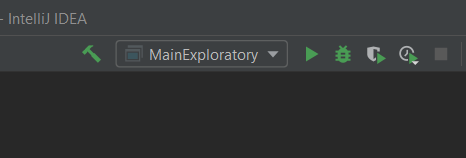
\includegraphics[scale=0.8]{exploratory_main_class}
	\caption{Main Class Perangkat Lunak Ekplorasi}
	\label{fig:pertama1}
\end{figure}

Setelah itu pilih menu \texttt{Edit Configurations..}, lalu isi parameter \texttt{Working directory} dengan lokasi \texttt{InputAnonymization.json}, contohnya pada Gambar \ref{fig:pertama2} \texttt{Working directory} diisi dengan nilai \path{D:\input\InputAnonymization.json}. Pada tahap ini langkah pertama telah selesai.

\begin{figure}[H]
	\centering
	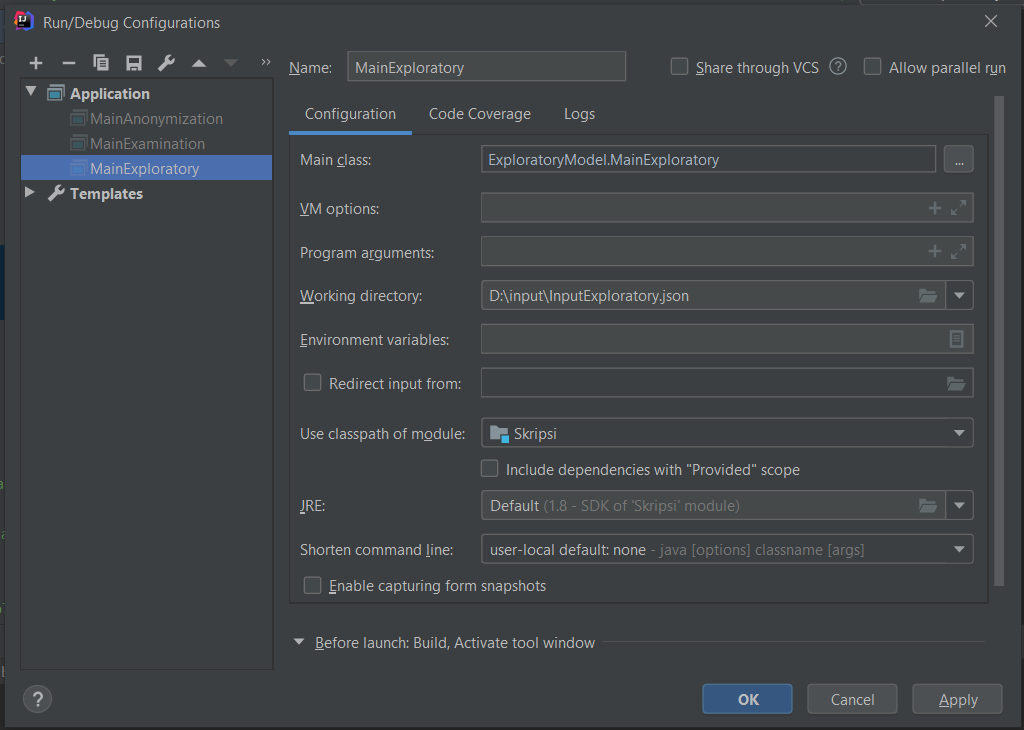
\includegraphics[scale=0.6]{exploratory_conf}
	\caption{Konfigurasi Parameter Perangkat Lunak Ekplorasi}
	\label{fig:pertama2}
\end{figure}

Langkah kedua adalah menjalankan perangkat lunak ekplorasi pada IntelIJ dengan memilih Main class pada sisi layar kiri layar, contohnya MainExploratory. Kemudian klik kanan pada Main class tersebut dan pilih menu \texttt{Run 'MainExploratory'}. Perangkat lunak akan menghasilkan output berupa tabel unik berdasarkan pemilihan \texttt{selected\_column} pada \texttt{InputExploratory.json}

\begin{figure}[H]
	\centering
	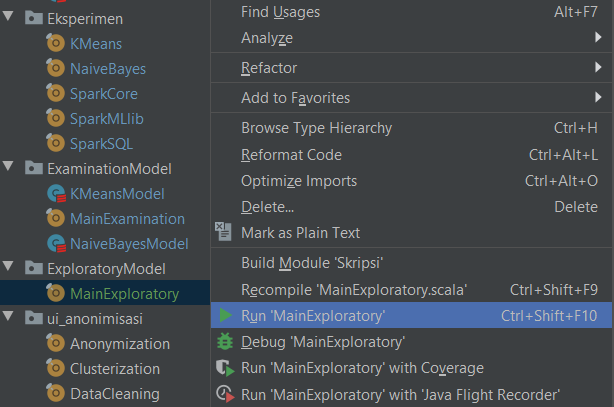
\includegraphics[scale=1]{exploratory_run}
	\caption{Menjalankan Perangkat Lunak Ekplorasi}
	\label{fig:pertama2}
\end{figure}

Langkah terakhir adalah menunggu proses komputasi sampai dengan selesai. Sebagai catatan semakin banyak data yang diolah, maka waktu komputasi akan semakin lama. Perangkat lunak eksplorasi yang telah berhasil menyelesaikan proses komputasinya ditandai dengan baris log seperti berikut \texttt{'Process finished with exit code 0}. Karena proses komputasi sudah selesai, output perangkat lunak eksplorasi sudah muncul berdasarkan \texttt{output\_path} pada \texttt{InputExploratory.json}

\begin{figure}[H]
	\centering
	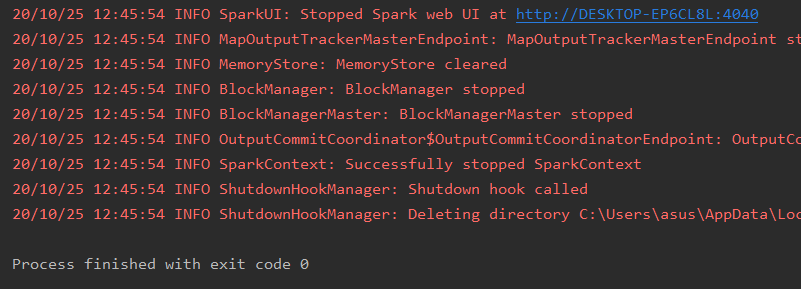
\includegraphics[scale=0.8]{exploratory_done}
	\caption{Log Perangkat Lunak Ekplorasi}
	\label{fig:pertama2}
\end{figure}

Output yang dihasilkan dari perangkat lunak eksplorasi dapat dilihat pada lokasi yang telah dicantumkan sebelumnya pada nilai \texttt{output\_path} JSON.  Sehingga ketika lokasi \texttt{output\_path} dibuka, maka akan tampak seperti Gamabar 1.1. Hasil eksplorasi nilai unik akan digunakan sebagai referensi mengisi nilai \texttt{domain\_generalization\_hierarchy} sebuah atribut tabel data pada \texttt{InputAnonymization.json}. Eksplorasi perlu dilakukan mengingat seluruh nilai atribut harus dapat diubah menjadi nilai anonimisasi. Output dapat dilihat ketika membuka file \texttt{part-000X-YYYYY.csv}.

\begin{figure}[H]
	\centering
	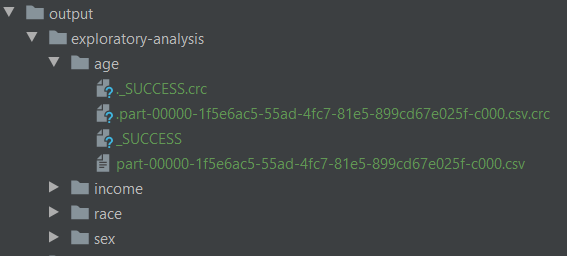
\includegraphics[scale=1]{exploratory_result}
	\caption{Folder Output Perangkat Lunak Ekplorasi}
	\label{fig:pertama2}
\end{figure}

Contoh output yang dihasilkan adalah tabel nilai unik dari atribut \texttt{Age}. Karena output disimpan dalam format CSV, baris pertama menyatakan nama kolom, sedangkan baris selanjutnya menyatakan nilai unik pada kolom tersebut.  Diketahui bahwa nilai unik atribut \texttt{Age} memiliki 5 jenis nilai unik.

\begin{figure}[H]
	\centering
	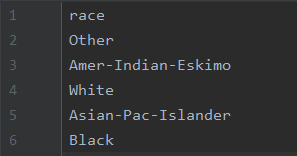
\includegraphics[scale=0.8]{exploratory_result2}
	\caption{Tabel Nilai Unik (Age)}
	\label{fig:pertama2}
\end{figure}

\noindent Listing 4 adalah contoh input JSON dengan nama \texttt{InputExploratory.json}:

\begin{lstlisting}[basicstyle=\ttfamily, frame=single,
	columns=fullflexible, keepspaces=true, breaklines=true, label=lst:pl_csv, caption=Data JSON untuk Perangkat Lunak Eksplorasi]
{
  "input_path": "D:/input/adult100k.csv",
  "output_path": "D:/output/exploratory-analysis/",
  "selected_column": [
      {
        "attrName": "age",
        "dataType": "numeric"
      },
      {
        "attrName": "race",
        "dataType": "category"
      },
      {
        "attrName": "sex",
        "dataType": "category"
      },
      {
        "attrName": "income",
        "dataType": "category"
      }
  ]
}
\end{lstlisting}

\subsubsection{Perangkat Lunak Anonimisasi}

Setelah mengeksekusi perangkat lunak eksplorasi untuk mencari tahu nilai unik pada setiap kolom quasi-identifier, pengujian akan dilanjutkan pada perangkat lunak anonimisasi untuk mencari tahu mengenai hasil pengelompokan data dengan algoritma Greedy k-member clustering.

\begin{figure}[H]
	\centering
	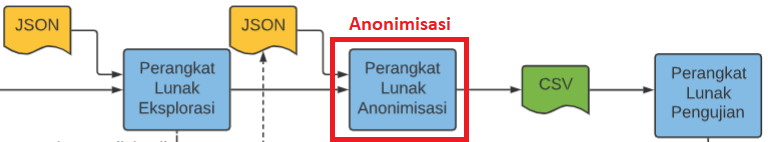
\includegraphics[scale=0.8]{diagram_aktivitas_bab5_1}
	\caption{Main Class Perangkat Lunak Ekplorasi}
	\label{fig:pertama1}
\end{figure}

Langkah pertama sebelum menjalankan perangkat lunak ekplorasi pada IntelIJ adalah mengisi parameter input. Caranya dengan menekan tombol selector Main class pada sisi layar kanan atas, contohnya pada \ref{fig:pertama1} tombol selector Main class yang ditekan bernama MainExploratory. 

\begin{figure}[H]
	\centering
	
\includegraphics[scale=0.9]{anonymization_main_class}
	\caption{Main Class Perangkat Lunak Ekplorasi}
	\label{fig:pertama1}
\end{figure}

\newpage
Setelah itu pilih menu \texttt{Edit Configurations..}, lalu isi parameter \texttt{Working directory} dengan lokasi \texttt{InputAnonymization.json}, contohnya pada Gambar \ref{fig:pertama2} \texttt{Working directory} diisi dengan nilai \path{D:\input\InputAnonymization.json}. Pada tahap ini langkah pertama telah selesai.

\begin{figure}[H]
	\centering
	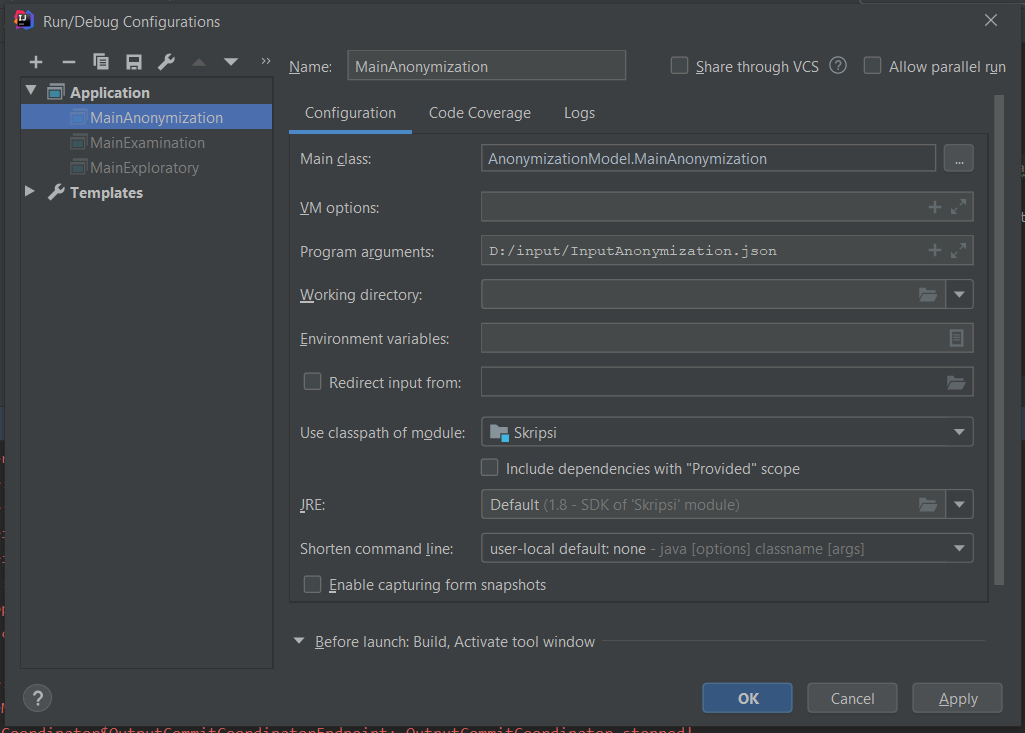
\includegraphics[scale=0.6]{anonymization_conf}
	\caption{Konfigurasi Parameter Perangkat Lunak Ekplorasi}
	\label{fig:pertama2}
\end{figure}

Langkah kedua adalah menjalankan perangkat lunak ekplorasi pada IntelIJ dengan memilih Main class pada sisi layar kiri layar, contohnya MainExploratory. Kemudian klik kanan pada Main class tersebut dan pilih menu \texttt{Run 'MainExploratory'}. Perangkat lunak akan menghasilkan output berupa tabel unik berdasarkan pemilihan \texttt{selected\_column} pada \texttt{InputExploratory.json}

\begin{figure}[H]
	\centering
	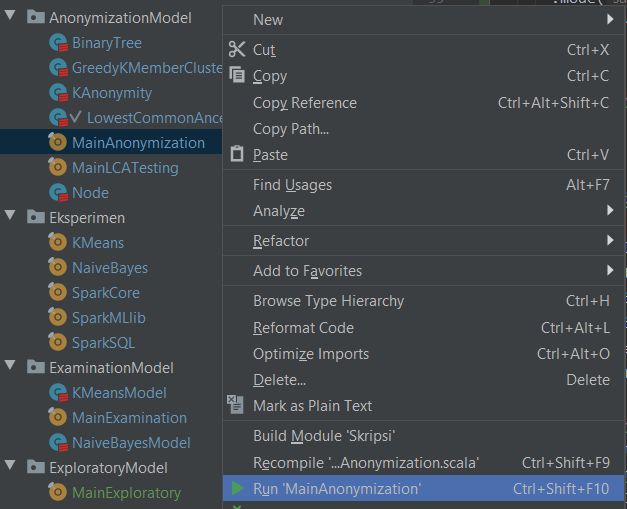
\includegraphics[scale=0.8]{anonymization_run}
	\caption{Menjalankan Perangkat Lunak Ekplorasi}
	\label{fig:pertama2}
\end{figure}

\newpage
Langkah terakhir adalah menunggu proses komputasi sampai dengan selesai. Sebagai catatan semakin banyak data yang diolah, maka waktu komputasi akan semakin lama. Perangkat lunak eksplorasi yang telah berhasil menyelesaikan proses komputasinya ditandai dengan baris log seperti berikut \texttt{'Process finished with exit code 0}. Karena proses komputasi sudah selesai, output perangkat lunak eksplorasi sudah muncul berdasarkan \texttt{output\_path} pada \texttt{InputExploratory.json}

\begin{figure}[H]
	\centering
	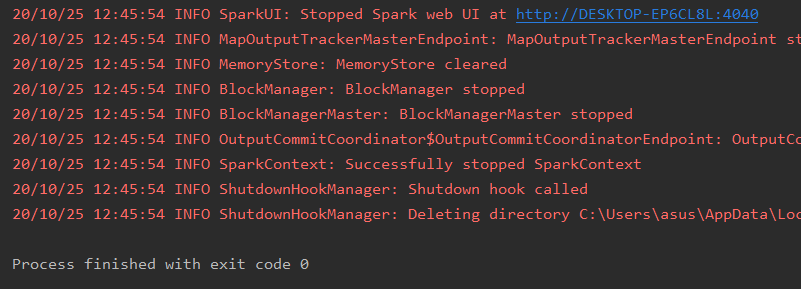
\includegraphics[scale=0.8]{exploratory_done}
	\caption{Log Perangkat Lunak Ekplorasi}
	\label{fig:pertama2}
\end{figure}

Output yang dihasilkan dari perangkat lunak eksplorasi dapat dilihat pada lokasi yang telah dicantumkan sebelumnya pada nilai \texttt{output\_path} JSON.  Sehingga ketika lokasi \texttt{output\_path} dibuka, maka akan tampak seperti Gamabar 1.1. Hasil eksplorasi nilai unik akan digunakan sebagai referensi mengisi nilai \texttt{domain\_generalization\_hierarchy} sebuah atribut tabel data pada \texttt{InputAnonymization.json}. Eksplorasi perlu dilakukan mengingat seluruh nilai atribut harus dapat diubah menjadi nilai anonimisasi. Output dapat dilihat ketika membuka file \texttt{part-000X-YYYYY.csv}.

\begin{figure}[H]
	\centering
	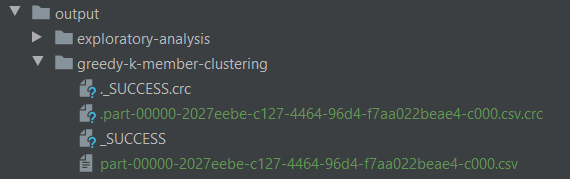
\includegraphics[scale=1]{greedy_result}
	\caption{Folder Output Perangkat Lunak Anonimisasi}
	\label{fig:pertama2}
\end{figure}

Contoh output yang dihasilkan adalah tabel pengolompokan data berdasarkan atribut quasi-identifier \texttt{age,race,sex,workclass,income}. Karena output disimpan dalam format CSV, baris pertama menyatakan nama kolom, sedangkan baris selanjutnya menyatakan nilai unik pada kolom tersebut. Diketahui bahwa masing-masing data sudah dikelompokan ke masing-masing cluster. Sampel membentuk 2 kelompok data, karena dipilih parameter k=2 pada InputAnonymization.json.

\begin{figure}[H]
	\centering
	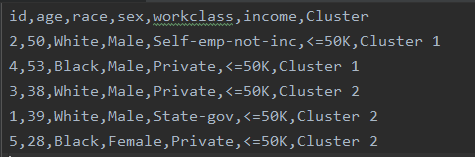
\includegraphics[scale=1]{greedy_result2}
	\caption{Tabel Pengelompokan Data}
	\label{fig:pertama2}
\end{figure}

\newpage
\noindent Listing \ref{lst:anonymization_json} adalah contoh input JSON dengan nama \texttt{InputAnonymization.json}:

\begin{lstlisting}[basicstyle=\ttfamily, frame=single,
	columns=fullflexible, keepspaces=true, breaklines=true, label=lst:anonymization_json, caption=Data JSON untuk Perangkat Lunak Eksplorasi]
{
  "k": 2,
  "num_sample_datas": 5,
  "input_path": "D:/input/adult100k.csv",
  "output_path": "D:/output/",
  "identifier": [
      {
        "attrName": "name",
        "dataType": "category"
      }
  ],
  "sensitive_identifier": [
      {
        "attrName": "income",
        "dataType": "category"
      }
  ],
  "quasi_identifier": [
      {
        "attrName": "age",
        "dataType": "numeric"
      },
      {
        "attrName": "race",
        "dataType": "category"
      },
      {
        "attrName": "sex",
        "dataType": "category"
      },
      {
        "attrName": "workclass",
        "dataType": "category"
      }
  ],
  "domain_generalization_hierarchy": {
      "race":[
          {
            "value": "Person",
            "parent": "Person",
            "level": "1",
            "position": "null"
          },
          {
            "value": "Oriental",
            "parent": "Person",
            "level": "2",
            "position": "left"
          },
          {
            "value": "General",
            "parent": "Person",
            "level": "2",
            "position": "right"
          },
          {
            "value": "Amer-Indian-Eskimo",
            "parent": "Oriental",
            "level": "3",
            "position": "left"
          },
          {
            "value": "Asian",
            "parent": "Oriental",
            "level": "3",
            "position": "right"
          },
          {
            "value": "White",
            "parent": "General",
            "level": "3",
            "position": "left"
          },
          {
            "value": "Black",
            "parent": "General",
            "level": "3",
            "position": "right"
          }
      ],
      "sex":[
          {
            "value": "Adult",
            "parent": "Adult",
            "level": "1",
            "position": "null"
          },
          {
            "value": "Female",
            "parent": "Adult",
            "level": "2",
            "position": "left"
          },
          {
            "value": "Male",
            "parent": "Adult",
            "level": "2",
            "position": "right"
          }
      ],
      "workclass":[
        {
          "value": "Employee",
          "parent": "Employee",
          "level": "1",
          "position": "null"
        },
        {
          "value": "Gov-employee",
          "parent": "Employee",
          "level": "2",
          "position": "left"
        },
        {
          "value": "Local-employee",
          "parent": "Employee",
          "level": "2",
          "position": "right"
        },
        {
          "value": "Gov",
          "parent": "Gov-employee",
          "level": "3",
          "position": "left"
        },
        {
          "value": "Other-gov",
          "parent": "Gov-employee",
          "level": "3",
          "position": "right"
        },
        {
          "value": "Self-emp",
          "parent": "Local-employee",
          "level": "3",
          "position": "left"
        },
        {
          "value": "Others",
          "parent": "Local-employee",
          "level": "3",
          "position": "right"
        },
        {
          "value": "State-gov",
          "parent": "Government",
          "level": "4",
          "position": "left"
        },
        {
          "value": "Federal-gov",
          "parent": "Government",
          "level": "4",
          "position": "right"
        },
        {
          "value": "Self-emp-not-inc",
          "parent": "Self-emp",
          "level": "4",
          "position": "left"
        },
        {
          "value": "Self-emp-inc",
          "parent": "Self-emp",
          "level": "4",
          "position": "right"
        },
        {
          "value": "Private",
          "parent": "Others",
          "level": "4",
          "position": "left"
        },
        {
          "value": "Never-worked",
          "parent": "Others",
          "level": "4",
          "position": "right"
        },
        {
          "value": "Local-gov",
          "parent": "Others-gov",
          "level": "4",
          "position": "left"
        },
        {
          "value": "Without-pay",
          "parent": "Others-gov",
          "level": "4",
          "position": "right"
        }
      ]
  }
}
\end{lstlisting}

\newpage
\subsubsection{Perangkat Lunak Pengujian}
Setelah mengeksekusi perangkat lunak eksplorasi untuk mencari tahu nilai unik pada setiap kolom quasi-identifier, pengujian akan dilanjutkan pada perangkat lunak anonimisasi untuk mencari tahu mengenai hasil pengelompokan data dengan algoritma Greedy k-member clustering.

\begin{figure}[H]
	\centering
	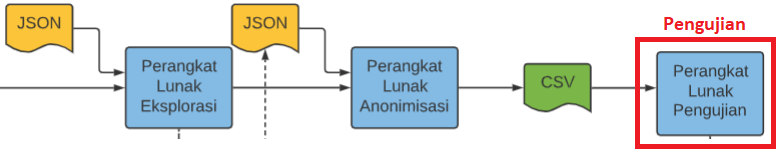
\includegraphics[scale=0.8]{diagram_aktivitas_bab5_2}
	\caption{Main Class Perangkat Lunak Ekplorasi}
	\label{fig:pertama1}
\end{figure}

Langkah pertama sebelum menjalankan perangkat lunak ekplorasi pada IntelIJ adalah mengisi parameter input. Caranya dengan menekan tombol selector Main class pada sisi layar kanan atas, contohnya pada \ref{fig:pertama1} tombol selector Main class yang ditekan bernama MainExploratory. 

\begin{figure}[H]
	\centering
	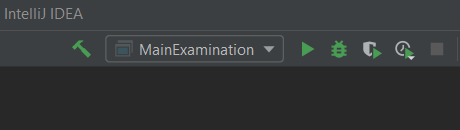
\includegraphics[scale=0.8]{examination_main_class}
	\caption{Main Class Perangkat Lunak Ekplorasi}
	\label{fig:pertama1}
\end{figure}

Setelah itu pilih menu \texttt{Edit Configurations..}, lalu isi parameter \texttt{Working directory} dengan lokasi \texttt{InputAnonymization.json}, contohnya pada Gambar \ref{fig:pertama2} \texttt{Working directory} diisi dengan nilai \path{D:\input\InputAnonymization.json}. Pada tahap ini langkah pertama telah selesai.

\begin{figure}[H]
	\centering
	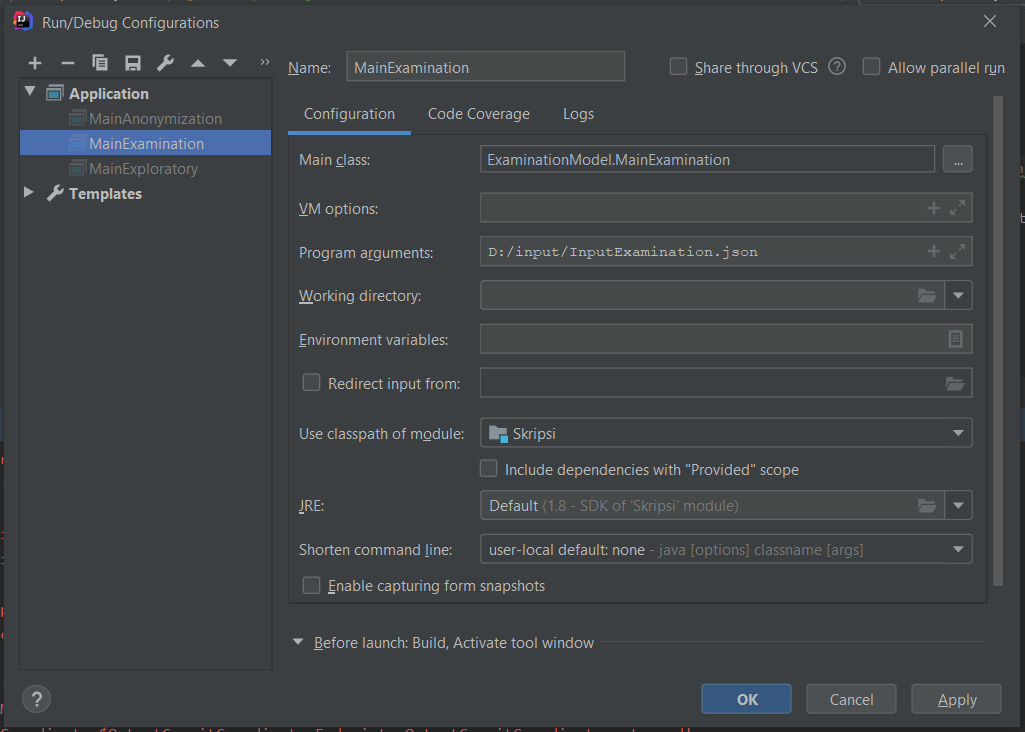
\includegraphics[scale=0.6]{examination_conf}
	\caption{Konfigurasi Parameter Perangkat Lunak Ekplorasi}
	\label{fig:pertama2}
\end{figure}

Langkah kedua adalah menjalankan perangkat lunak ekplorasi pada IntelIJ dengan memilih Main class pada sisi layar kiri layar, contohnya MainExploratory. Kemudian klik kanan pada Main class tersebut dan pilih menu \texttt{Run 'MainExploratory'}. Perangkat lunak akan menghasilkan output berupa tabel unik berdasarkan pemilihan \texttt{selected\_column} pada \texttt{InputExploratory.json}

\begin{figure}[H]
	\centering
	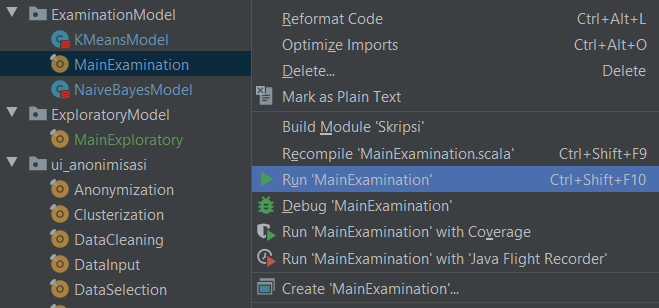
\includegraphics[scale=1]{examination_run}
	\caption{Menjalankan Perangkat Lunak Ekplorasi}
	\label{fig:pertama2}
\end{figure}

Langkah terakhir adalah menunggu proses komputasi sampai dengan selesai. Sebagai catatan semakin banyak data yang diolah, maka waktu komputasi akan semakin lama. Perangkat lunak eksplorasi yang telah berhasil menyelesaikan proses komputasinya ditandai dengan baris log seperti berikut \texttt{'Process finished with exit code 0}. Karena proses komputasi sudah selesai, output perangkat lunak eksplorasi sudah muncul berdasarkan \texttt{output\_path} pada \texttt{InputExploratory.json}

\begin{figure}[H]
	\centering
	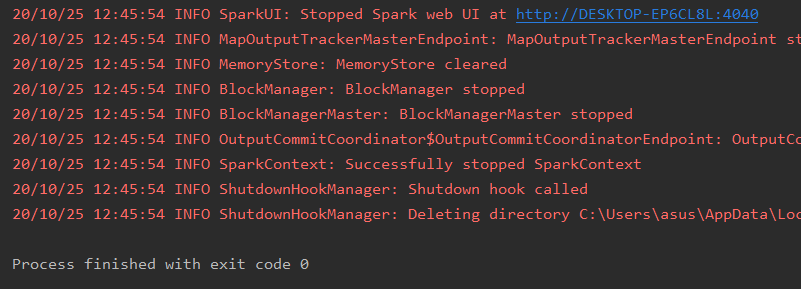
\includegraphics[scale=0.8]{exploratory_done}
	\caption{Log Perangkat Lunak Ekplorasi}
	\label{fig:pertama2}
\end{figure}

Output yang dihasilkan dari perangkat lunak eksplorasi dapat dilihat pada lokasi yang telah dicantumkan sebelumnya pada nilai \texttt{output\_path} JSON.  Sehingga ketika lokasi \texttt{output\_path} dibuka, maka akan tampak seperti Gamabar 1.1. Hasil eksplorasi nilai unik akan digunakan sebagai referensi mengisi nilai \texttt{domain\_generalization\_hierarchy} sebuah atribut tabel data pada \texttt{InputAnonymization.json}. Eksplorasi perlu dilakukan mengingat seluruh nilai atribut harus dapat diubah menjadi nilai anonimisasi. Output dapat dilihat ketika membuka file \texttt{part-000X-YYYYY.csv}.

\begin{figure}[H]
	\centering
	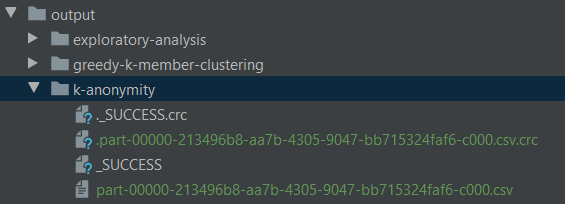
\includegraphics[scale=1]{examination_result}
	\caption{Folder Output Perangkat Lunak Ekplorasi}
	\label{fig:pertama2}
\end{figure}

Contoh output yang dihasilkan adalah tabel anonimisasi data berdasarkan atribut quasi-identifier \texttt{age,race,sex,workclass,income}. Karena output disimpan dalam format CSV, baris pertama menyatakan nama kolom, sedangkan baris selanjutnya menyatakan nilai unik pada kolom tersebut. Diketahui bahwa masing-masing data sudah dianonimisasi berdasarkan Domain Generalization Hierarchy. Sampel sudah membentuk equivalence class, dimana sebuah data menjadi sulit dibedakan dengan data lainnya. Hal ini membuktikan prinsip k-anonymity telah tercapai pada penelitian ini.

\begin{figure}[H]
	\centering
	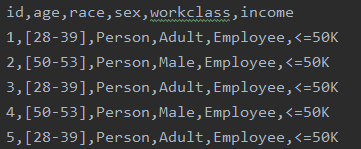
\includegraphics[scale=1.]{examination_result2}
	\caption{Tabel Nilai Unik (Age)}
	\label{fig:pertama2}
\end{figure}

\noindent Listing 4 adalah contoh input JSON dengan nama \texttt{InputExamination.json}:

\begin{lstlisting}[basicstyle=\ttfamily, frame=single,
	columns=fullflexible, keepspaces=true, breaklines=true, label=lst:pl_csv, caption=Data JSON untuk Perangkat Lunak Eksplorasi]
{
  "input_path": "D:/input/adult100k.csv",
  "output_path": "D:/output/",
  "selected_column": [
      {
        "attrName": "age",
        "dataType": "numeric"
      },
      {
        "attrName": "race",
        "dataType": "category"
      },
      {
        "attrName": "sex",
        "dataType": "category"
      },
      {
        "attrName": "income",
        "dataType": "category"
      }
  ]
}
{
  "input_path": "D:/input/adult100k.csv",
  "output_path": "D:/output/",
  "model_name": "k_means",
  "selected_column": [
      {
        "attrName": "age",
        "dataType": "numeric"
      },
      {
        "attrName": "race",
        "dataType": "category"
      },
      {
        "attrName": "sex",
        "dataType": "category"
      },
      {
        "attrName": "income",
        "dataType": "category"
      }
  ],
  "k_means": {
      "k": 2
  },
  "naive_bayes": {
      "label": "income",
      "training_set": 0.7,
      "test_set": 0.3
  }
}
\end{lstlisting}



\subsection{Hadoop Cluster dengan Terminal Ubuntu}
Pengujian ini dilakukan menggunakan Hadoop cluster dengan 10 slaves node yang dapat digunakan untuk proses komputasi. Hasil pengujian ini memiliki hasil output yang sama jika dijalankan pada komputer lokal. Perbedaanya terletak pada jumlah komputer yang melakukan komputasi. Apabila menggunakan Hadoop cluster, waktu komputasi untuk memproses ukuran data yang besar dapat dikurangi, karena komputasi dilakukan secara paralel terhadap 10 slaves node. Perintah untuk melakukan eksekusi Spark dapat ditulis menggunakan terminal Ubuntu.

\begin{figure}[H]
	\centering
	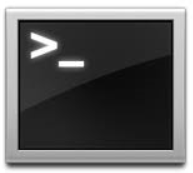
\includegraphics[scale=0.8]{terminal}
	\caption{Terminal Ubuntu}
	\label{fig:pertama0}
\end{figure}

\newpage
\noindent Berikut adalah spesifikasi slaves node pada Hadoop cluster:

\begin{figure}[H]
	\centering
	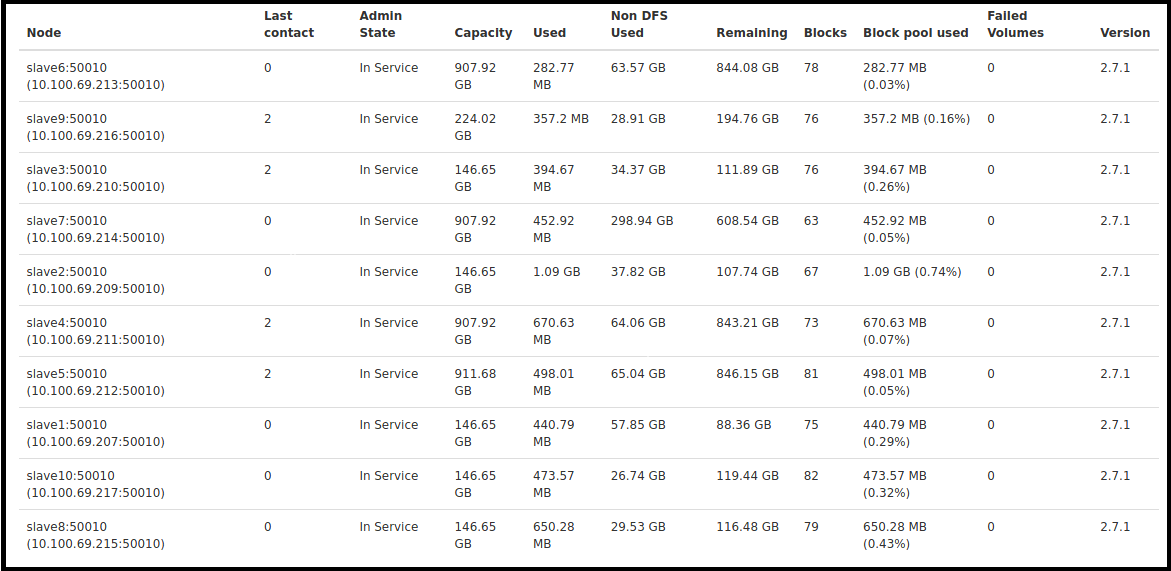
\includegraphics[scale=0.66]{datanode_info1}
	\caption{Spesifikasi Slaves Node }
	\label{fig:pertama0}
\end{figure}

\begin{itemize}
\item Node adalah nama dan alamat slaves node yang tersedia pada Hadoop cluster.
\item Capacity adalah kapasitas penyimpanan data pada masing-masing slaves node.
\item Used adalah jumlah kapasitas yang terpakai pada masing-masing slaves node.
\item Remaining adalah sisa kapasitas penyimpanan pada masing-masing slaves node.
\item Version adalah versi hadoop yang dipasang pada masing-masing slaves node.
\end{itemize}

\subsubsection{Perangkat Lunak Eksplorasi}

Langkah pertama sebelum menjalankan perangkat lunak ekplorasi pada CLI adalah menyimpan data input pada sistem HDFS. Data input yang dibutuhkan antara lain dataset \texttt{adult100k.csv} dan parameter program \texttt{InputExploratory.json}. Listing 1 adalah perintah untuk membuat folder dan menyimpan data input pada HDFS. Hasil folder dan file yang disimpan pada HDFS dapat dilihat menggunakan browser dengan alamat \path{http://10.100.69.101:50070/}.

\begin{lstlisting}[basicstyle=\ttfamily, frame=single,
	columns=fullflexible, keepspaces=true, breaklines=true, label=lst:pl_csv, caption=Perintah Spark untuk Perangkat Lunak Eksplorasi]
// Perintah untuk membuat folder di HDFS
hadoop fs -mkdir /<nama folder HDFS>

// Perintah untuk menyimpan file adult100k.csv di HDFS
hadoop fs -put /home/hduser/<nama folder>/<nama file>.csv /<nama folder HDFS>/

// Perintah untuk menyimpan file InputAnonymization.json di HDFS
hadoop fs -put /home/hduser/<nama folder>/<nama file>.json /<nama folder HDFS>/

// Perintah untuk menghapus sebuah folder pada HDFS
hadoop fs -rm -r -f /<nama folder HDFS>

\end{lstlisting}

\newpage
Langkah kedua adalah memastikan bahwa file sudah ditempatkan pada folder dengan nama yang sesuai. Hal ini perlu diperhatikan, karena jika terjadi kesalahan input pada nama file atau nama folder, program dapat menampilkan pesan error. Gambar 1 adalah contoh penempatan file pada folder HDFS dengan benar karena tidak ada kesalahan penulisan nama.

\begin{figure}[H]
	\centering
	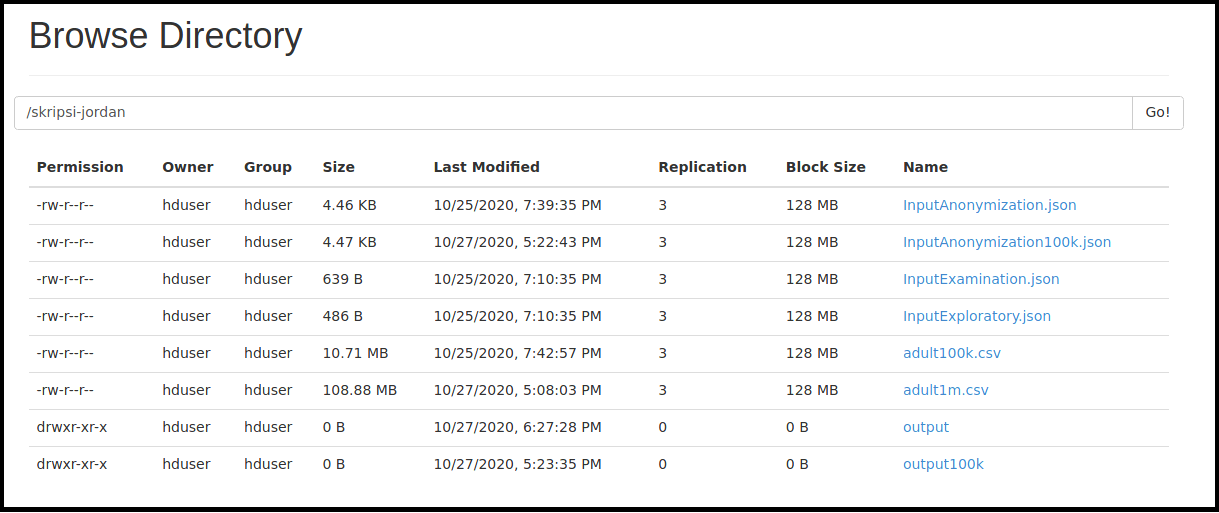
\includegraphics[scale=0.5]{hc_langkah2}
	\caption{File Input Eksplorasi HDFS}
	\label{fig:pertama2}
\end{figure}

Langkah ketiga adalah melakukan eksekusi perangkat lunak eksplorasi menggunakan perintah Spark. Listing 1 adalah contoh perintah eksekusi pada Spark. Format \texttt{\textemdash\textemdash class ExploratoryModel. MainExploratory} artinya menunjukan kelas Main yang dieksekusi bernama \texttt{MainExploratory} pada package \texttt{ExploratoryModel}. Format \texttt{\textemdash\textemdash master yarn} menunjukan bahwa program dieksekusi pada sebuah cluster komputer. Format \path{/home/hduser/skripsi-stephen/skripsi.jar} menunjukan lokasi JAR pada komputer. Format \path{/skripsi-jordan/InputExploratory.json} menunjukan lokasi JSON pada HDFS. Pada tahap ini, perintah Spark siap untuk dieksekusi.

\begin{lstlisting}[basicstyle=\ttfamily, frame=single,
	columns=fullflexible, keepspaces=true, breaklines=true, label=lst:pl_csv, caption=Perintah Eksekusi Spark]
spark-submit --class ExploratoryModel.MainExploratory --master yarn /home/hduser/skripsi-stephen/skripsi.jar /skripsi-jordan/InputExploratory.json

\end{lstlisting}

\vspace{0.3cm}
Langkah terakhir adalah menunggu proses komputasi sampai dengan selesai.  Perangkat lunak eksplorasi yang telah berhasil menyelesaikan proses komputasinya  pada command line ditandai dengan baris log seperti Gambar 5.25: \texttt{'Stopped Spark Web UI at \path{http://master:4040}'}. Setelah proses komputasi selesai, maka output perangkat lunak eksplorasi sudah disimpan pada HDFS dengan lokasi sebagai berikut \path{/skripsi-jordan/output/exploratory-analysis}

\begin{figure}[H]
	\centering
	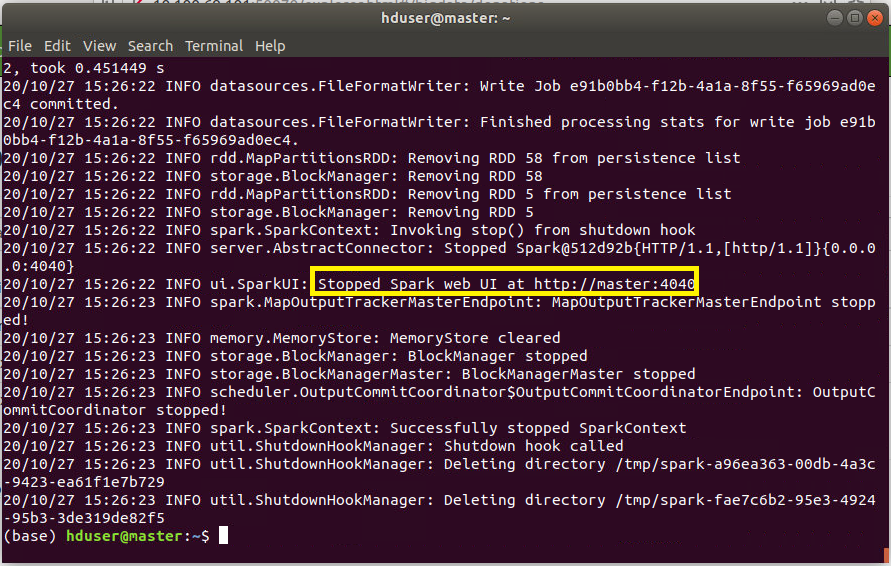
\includegraphics[scale=0.5]{hc_langkah5}
	\caption{Log Perangkat Lunak Ekplorasi}
	\label{fig:pertama2}
\end{figure}

Ketika lokasi output pada HDFS dibuka, maka akan tampak seperti Gambar 1.1. Hasil eksplorasi nilai unik akan digunakan sebagai referensi mengisi nilai \texttt{domain\_generalization\_hierarchy} sebuah atribut tabel data pada \texttt{InputExploratory.json}. Eksplorasi perlu dilakukan mengingat seluruh nilai atribut harus dapat diubah menjadi nilai anonimisasi. Gambar 5.26 menujukan lokasi folder nilai unik untuk masing-masing atribut. Gambar 5.27 menujukan  lokasi output disimpan \path{/skripsi-jordan/exploratory-analysis/workclass/part-000X-YYYYY.csv}.

\begin{figure}[H]
	\centering
	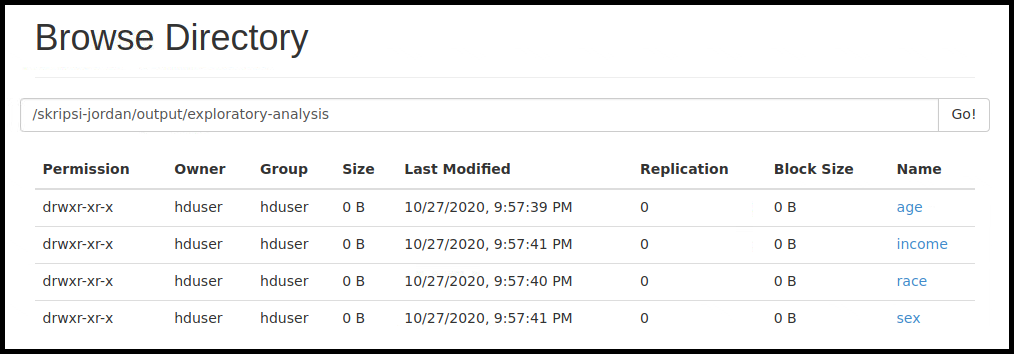
\includegraphics[scale=0.6]{hc_exploratory1}
	\caption{Folder HDFS Hasil Ekplorasi}
	\label{fig:pertama2}
\end{figure}

\begin{figure}[H]
	\centering
	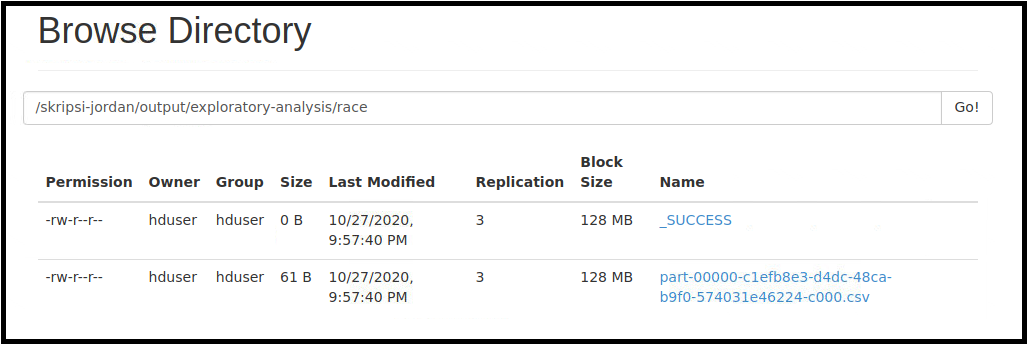
\includegraphics[scale=0.6]{hc_exploratory2}
	\caption{Folder HDFS Hasil Ekplorasi Atribut \texttt{Race}}
	\label{fig:pertama2}
\end{figure}

Contoh output yang dihasilkan adalah tabel nilai unik dari atribut \texttt{Race}. Karena output disimpan dalam format CSV, baris pertama menyatakan nama kolom, sedangkan baris selanjutnya menyatakan nilai unik. Gambar 5.28 menunjukan \texttt{Race} memiliki 5 jenis nilai unik.

\begin{figure}[H]
	\centering
	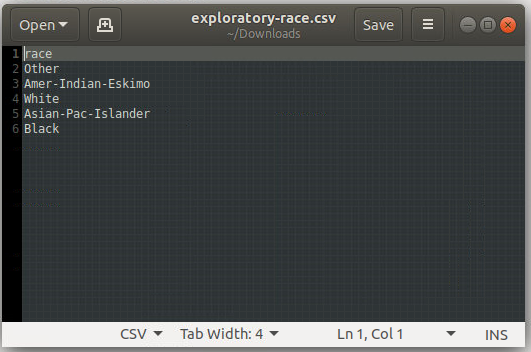
\includegraphics[scale=0.9]{hc_exploratory3}
	\caption{Hasil Eksplorasi pada Atribut Race}
	\label{fig:pertama2}
\end{figure}

\newpage
\subsubsection{Perangkat Lunak Anonimisasi}
Langkah pertama sebelum menjalankan perangkat lunak ekplorasi pada CLI adalah menyimpan data input pada sistem HDFS. Data input yang dibutuhkan antara lain dataset \texttt{adult100k.csv} dan parameter program \texttt{InputExploratory.json}. Listing 1 adalah perintah untuk membuat folder dan menyimpan data input pada HDFS. Hasil folder dan file yang disimpan pada HDFS dapat dilihat menggunakan browser dengan alamat \path{http://10.100.69.101:50070/}.

\begin{lstlisting}[basicstyle=\ttfamily, frame=single,
	columns=fullflexible, keepspaces=true, breaklines=true, label=lst:pl_csv, caption=Perintah Spark untuk Perangkat Lunak Anonimisasi]
// Perintah untuk membuat folder di HDFS
hadoop fs -mkdir /<nama folder HDFS>

// Perintah untuk menyimpan file adult100k.csv di HDFS
hadoop fs -put /home/hduser/<nama folder>/<nama file>.csv /<nama folder HDFS>/

// Perintah untuk menyimpan file InputAnonymization.json di HDFS
hadoop fs -put /home/hduser/<nama folder>/<nama file>.json /<nama folder HDFS>/

// Perintah untuk menghapus sebuah folder pada HDFS
hadoop fs -rm -r -f /<nama folder HDFS>

\end{lstlisting}

\vspace{0.3cm}
Langkah kedua adalah memastikan bahwa file sudah ditempatkan pada folder dengan nama yang sesuai. Hal ini perlu diperhatikan, karena jika terjadi kesalahan input pada nama file atau nama folder, program dapat menampilkan pesan error. Gambar 1 adalah contoh penempatan file pada folder HDFS dengan benar karena tidak ada kesalahan penulisan nama.

\begin{figure}[H]
	\centering
	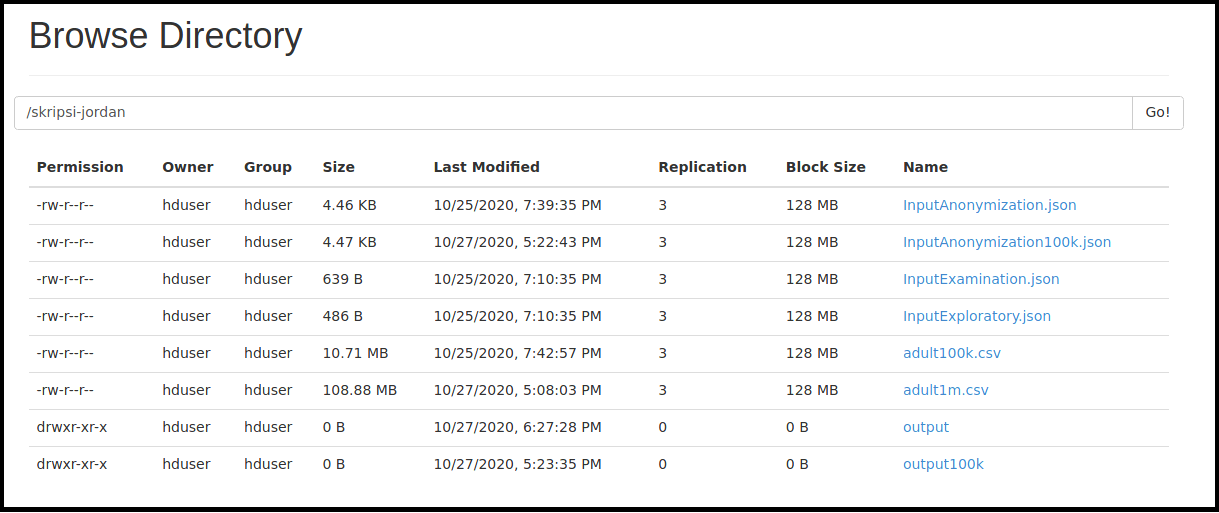
\includegraphics[scale=0.63]{hc_langkah2}
	\caption{File Input Anonimisasi HDFS}
	\label{fig:pertama2}
\end{figure}

Langkah ketiga adalah melakukan eksekusi perangkat lunak eksplorasi menggunakan perintah Spark. Listing 1 adalah contoh perintah eksekusi pada Spark. Format \texttt{\textemdash\textemdash class AnonymizationModel. MainAnonymization} artinya menunjukan kelas Main yang dieksekusi bernama \texttt{MainAnonymization} pada package \texttt{AnonymizationModel}. Format \texttt{\textemdash\textemdash master yarn} menunjukan bahwa program dieksekusi pada sebuah cluster komputer. Format \path{/home/hduser/skripsi-stephen/skripsi.jar} menunjukan lokasi JAR pada komputer. Format \path{/skripsi-jordan/InputAnonymization100k.json} menunjukan lokasi JSON pada HDFS. Pada tahap ini, perintah siap dieksekusi.

\newpage
\begin{lstlisting}[basicstyle=\ttfamily, frame=single,
	columns=fullflexible, keepspaces=true, breaklines=true, label=lst:pl_csv, caption=Perintah Eksekusi Spark]
spark-submit --class AnonymizationModel.MainAnonymization --master yarn /home/hduser/skripsi-stephen/skripsi.jar /skripsi-jordan/InputAnonymization100k.json

\end{lstlisting}

\vspace{0.3cm}
Langkah terakhir adalah menunggu proses komputasi sampai dengan selesai.  Perangkat lunak eksplorasi yang telah berhasil menyelesaikan proses komputasinya  pada command line ditandai dengan baris log seperti Gambar 5.25: \texttt{'Stopped Spark Web UI at \path{http://master:4040}'}. Setelah proses komputasi selesai, maka output perangkat lunak anonimisasi telah tersimpan pada HDFS. Hasil pengelompokan data disimpan pada lokasi HDFS sebagai berikut \path{/skripsi-jordan/output/greedy-k-member-clustering}, sedangkan hasil anonimisasi data disimpan pada lokasi HDFS sebagai berikut  \path{/skripsi-jordan/output/k-anonymity}.

\begin{figure}[H]
	\centering
	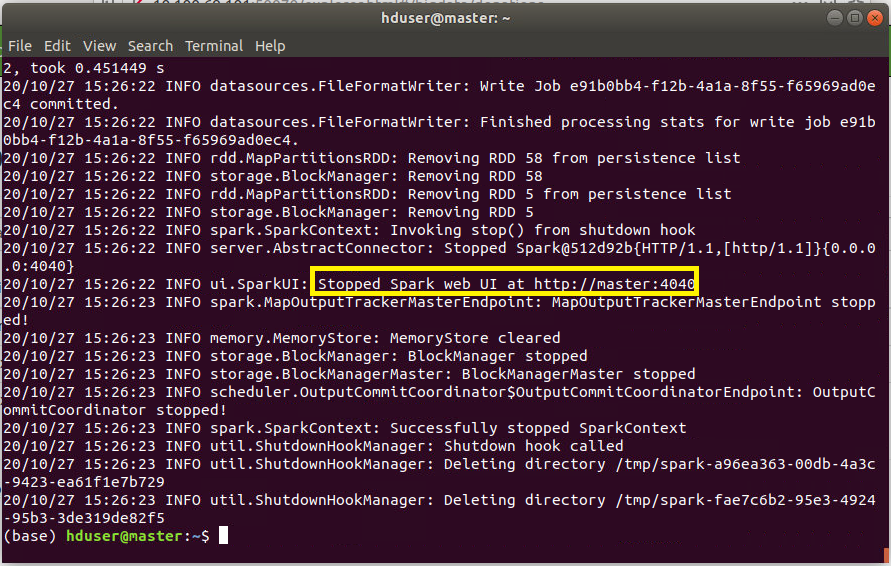
\includegraphics[scale=0.7]{hc_langkah5}
	\caption{Log Perangkat Lunak Anonimisasi}
	\label{fig:pertama2}
\end{figure}

Ketika lokasi output pada HDFS dibuka, maka akan tampak seperti Gambar 1.1. Hasil eksplorasi nilai unik akan digunakan sebagai referensi mengisi nilai \texttt{domain\_generalization\_hierarchy} sebuah atribut tabel data pada \texttt{InputAnonymization.json}. Gambar 5.27 menujukan hasil pengelompokan data pada \path{/skripsi-jordan/greedy-k-member-clustering/part-000X-YYYYY.csv}. Gambar 5.28 menujukan hasil pengelompokan data pada \path{/skripsi-jordan/k-anonymity/part-000X-YYYYY.csv}. Untuk membuka hasil output, maka CSV harus diunduh terlebih dahulu.

\begin{figure}[H]
	\centering
	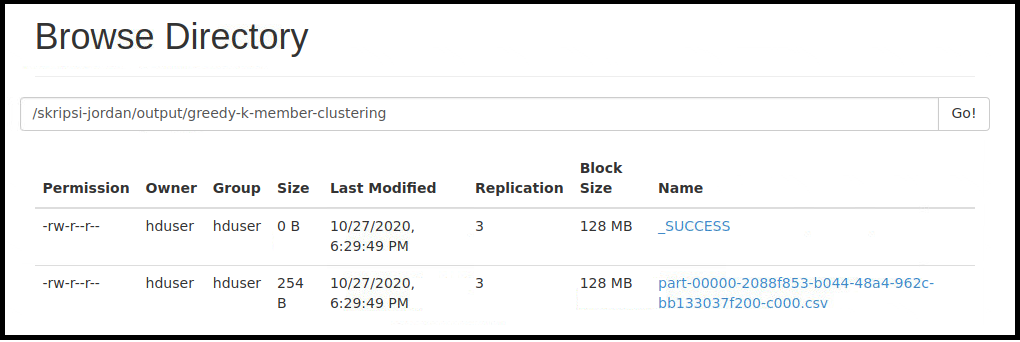
\includegraphics[scale=0.65]{hc_greedy2}
	\caption{Folder HDFS Hasil Pengelompokan Data}
	\label{fig:pertama2}
\end{figure}

\begin{figure}[H]
	\centering
	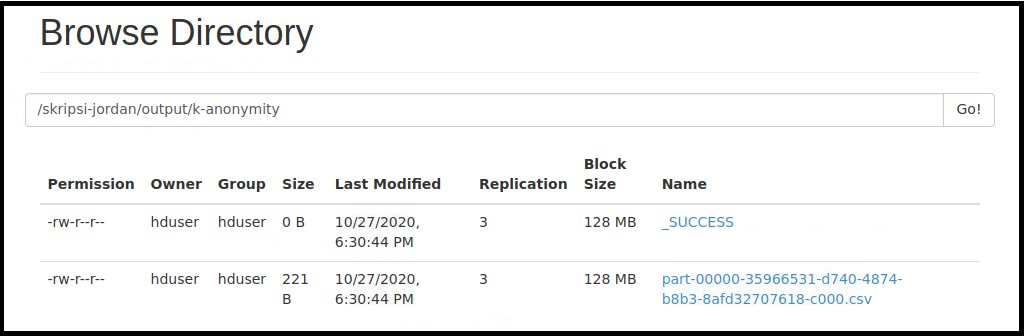
\includegraphics[scale=0.65]{hc_kanonymity2}
	\caption{Folder HDFS Hasil Anonimisasi Data}
	\label{fig:pertama2}
\end{figure}

Contoh output yang dihasilkan adalah tabel pengelompokan data dan tabel anonimisasi data. Karena output disimpan dalam format CSV, baris pertama menyatakan nama kolom, sedangkan baris selanjutnya menyimpan data. Gambar 5.33 menunjukan hasil pengelompokan data. Gambar 5.33 menunjukan hasil anonimisasi data. Output disimpan dalam format CSV.

\begin{figure}[H]
	\centering
	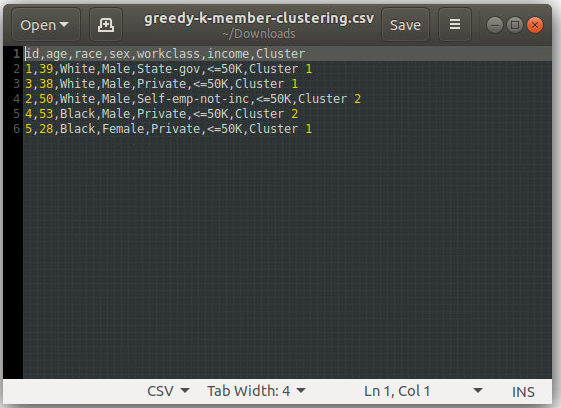
\includegraphics[scale=0.8]{hc_greedy1}
	\caption{Hasil Pengelompokan Greedy k-member clustering}
	\label{fig:pertama2}
\end{figure}

\begin{figure}[H]
	\centering
	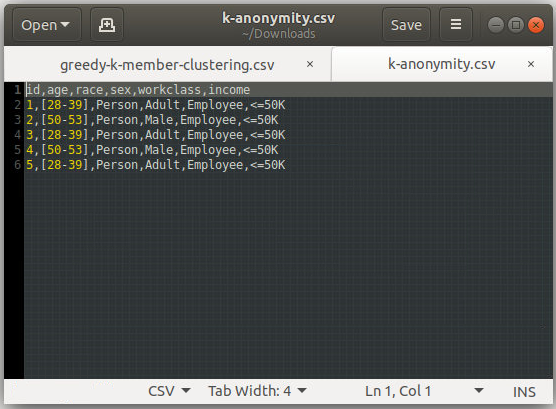
\includegraphics[scale=0.8]{hc_kanonymity1}
	\caption{Hasil Anonimisasi K-Anonymity}
	\label{fig:pertama2}
\end{figure}

\newpage
\subsubsection{Perangkat Lunak Pengujian}
Langkah pertama sebelum menjalankan perangkat lunak pengujian pada CLI adalah menyimpan data input pada sistem HDFS. Data input yang dibutuhkan antara lain dataset \texttt{adult100k.csv} dan parameter program \texttt{InputExploratory.json}. Listing 1 adalah perintah untuk membuat folder dan menyimpan data input pada HDFS. Hasil folder dan file yang disimpan pada HDFS dapat dilihat menggunakan browser dengan alamat \path{http://10.100.69.101:50070/}.

\begin{lstlisting}[basicstyle=\ttfamily, frame=single,
	columns=fullflexible, keepspaces=true, breaklines=true, label=lst:pl_csv, caption=Perintah Spark untuk Perangkat Lunak Pengujian]
// Perintah untuk membuat folder di HDFS
hadoop fs -mkdir /<nama folder HDFS>

// Perintah untuk menyimpan file adult100k.csv di HDFS
hadoop fs -put /home/hduser/<nama folder>/<nama file>.csv /<nama folder HDFS>/

// Perintah untuk menyimpan file InputAnonymization.json di HDFS
hadoop fs -put /home/hduser/<nama folder>/<nama file>.json /<nama folder HDFS>/

// Perintah untuk menghapus sebuah folder pada HDFS
hadoop fs -rm -r -f /<nama folder HDFS>

\end{lstlisting}

\vspace{0.4cm}
Langkah kedua adalah memastikan bahwa file sudah ditempatkan pada folder dengan nama yang sesuai. Hal ini perlu diperhatikan, karena jika terjadi kesalahan input pada nama file atau nama folder, program dapat menampilkan pesan error. Gambar 1 adalah contoh penempatan file pada folder HDFS dengan benar karena tidak ada kesalahan penulisan nama.

\begin{figure}[H]
	\centering
	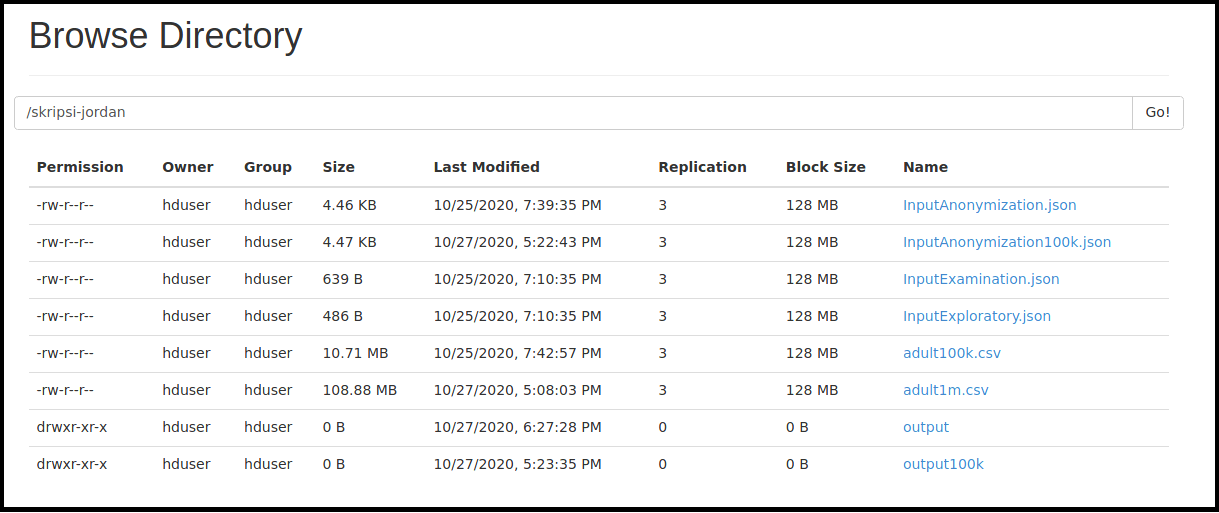
\includegraphics[scale=0.63]{hc_langkah2}
	\caption{File Input Pengujian HDFS}
	\label{fig:pertama2}
\end{figure}

Langkah ketiga adalah melakukan eksekusi perangkat lunak pengujian menggunakan perintah Spark. Listing 1 adalah contoh perintah eksekusi pada Spark. Format \texttt{\textemdash\textemdash class ExaminationModel. MainAnonymization} artinya menunjukan kelas Main yang dieksekusi bernama \texttt{MainAnonymization} pada package \texttt{ExaminationModel}. Format \texttt{\textemdash\textemdash master yarn} menunjukan bahwa program dieksekusi pada sebuah cluster komputer. Format \path{/home/hduser/skripsi-stephen/skripsi.jar} menunjukan lokasi JAR pada komputer. Format \path{/skripsi-jordan/InputKMeans.json} menunjukan lokasi JSON  pada HDFS untuk pemodelan k-means dan format \path{/skripsi-jordan/InputNaiveBayes.json} menunjukan lokasi JSON pada HDFS untuk pemodelan naive bayes. 

\newpage

\begin{lstlisting}[basicstyle=\ttfamily, frame=single,
	columns=fullflexible, keepspaces=true, breaklines=true, label=lst:pl_csv, caption=Perintah Eksekusi Spark]
spark-submit --class ExaminationModel.MainExamination --master yarn /home/hduser/skripsi-stephen/skripsi.jar /skripsi-jordan/InputExamination.json

\end{lstlisting}

\vspace{0.3cm}
Langkah terakhir adalah menunggu proses komputasi sampai dengan selesai.  Perangkat lunak pengujian yang telah berhasil menyelesaikan proses komputasinya  pada command line ditandai dengan baris log seperti Gambar 5.25: \texttt{'Stopped Spark Web UI at \path{http://master:4040}'}. Setelah proses komputasi selesai, maka hasil pengujian k-means disimpan sebagai format CSV pada lokasi HDFS berikut \path{/skripsi-jordan/output/k-means}, sedangkan hasil pemodelan naive bayes disimpan sebagai format CSV pada lokasi HDFS berikut \path{/skripsi-jordan/output/naive-bayes}.

\begin{figure}[H]
	\centering
	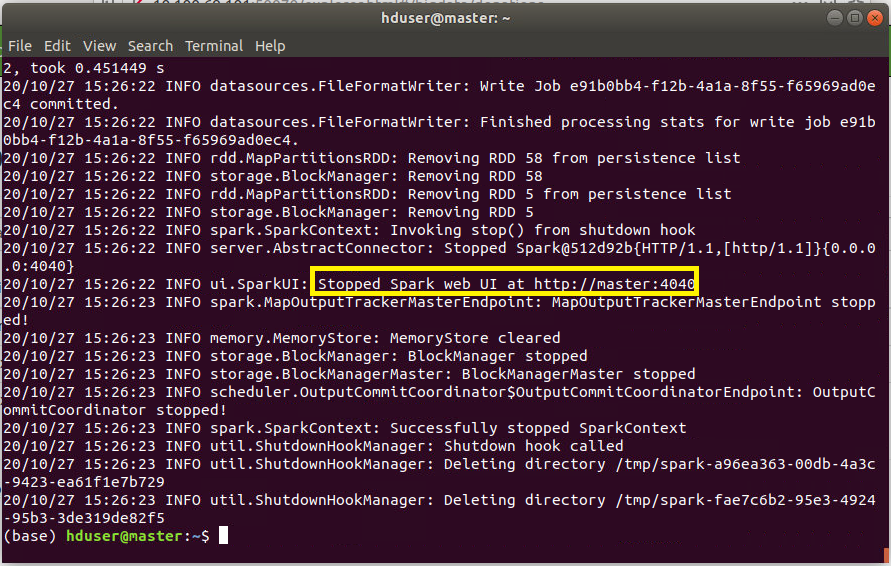
\includegraphics[scale=0.7]{hc_langkah5}
	\caption{Log Perangkat Lunak Pengujian}
	\label{fig:pertama2}
\end{figure}

Ketika lokasi output pada HDFS dibuka, maka akan tampak seperti Gambar 1.1. Hasil eksplorasi nilai unik akan digunakan sebagai referensi mengisi nilai \texttt{domain\_generalization\_hierarchy} sebuah atribut tabel data pada \texttt{InputAnonymization.json}. Eksplorasi perlu dilakukan mengingat seluruh nilai atribut harus dapat diubah menjadi nilai anonimisasi. Gambar 5.26 menujukan lokasi HDFS yang menyimpan hasil pengolompokan data pada CSV \path{/skripsi-jordan/output/naive-bayes/part-000X-YYYYY.csv}. Gambar 5.27 menujukan lokasi HDFS yang menyimpan hasil klasifikasi data pada CSV \path{/skripsi-jordan/output/naive-bayes/part-000X-YYYYY.csv}.

\begin{figure}[H]
	\centering
	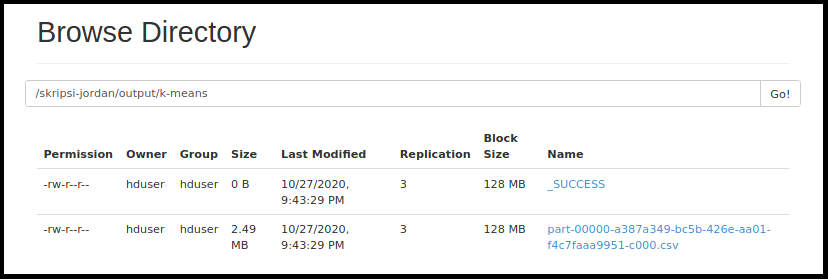
\includegraphics[scale=0.8]{hc_examination_kmeans2}
	\caption{Folder HDFS Hasil Pengelompokan K-Means}
	\label{fig:pertama2}
\end{figure}

\begin{figure}[H]
	\centering
	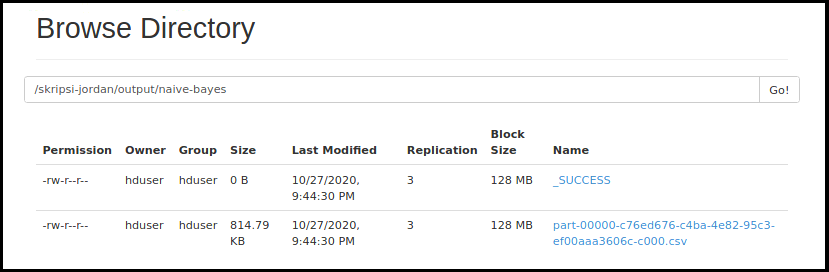
\includegraphics[scale=0.8]{hc_examination_naivebayes2}
	\caption{Folder HDFS Hasil Klasifikasi Naive Bayes}
	\label{fig:pertama2}
\end{figure}

Contoh output yang dihasilkan adalah tabel pengelompokan data k-means dan tabel klasifikasi data naive bayes. Karena output disimpan dalam format CSV, baris pertama menyatakan nama kolom, sedangkan baris selanjutnya menyatakan data. Gambar 5.28 menunjukan tabel pengelompokan data k-means. Gambar 5.29 menunjukan tabel klasifikasi data naive bayes.

\begin{figure}[H]
	\centering
	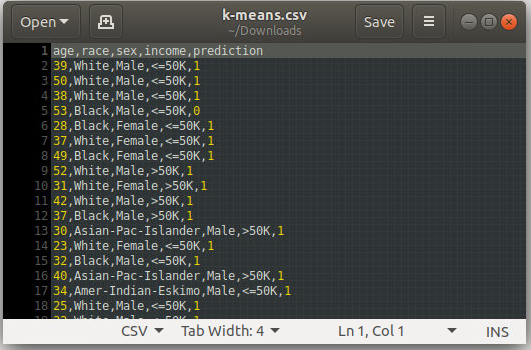
\includegraphics[scale=0.9]{hc_examination_kmeans}
	\caption{Hasil Pengelompokan K-Means}
	\label{fig:pertama2}
\end{figure}

\begin{figure}[H]
	\centering
	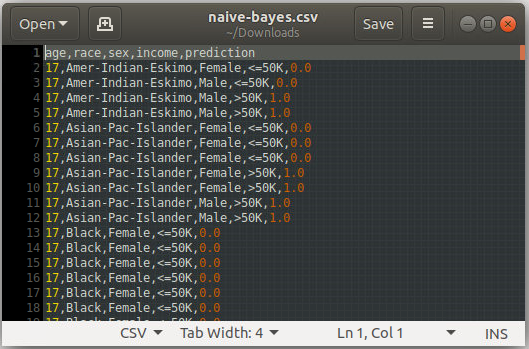
\includegraphics[scale=0.9]{hc_examination_naivebayes}
	\caption{Hasil Klasifikasi Naive Bayes}
	\label{fig:pertama2}
\end{figure}

\section{Pengujian}
Pengujian pada penelitian ini dibagi menjadi dua tahap, yaitu pengujian fungsional dan pengujian eksperimental. Pengujian fungsional bertujuan untuk melihat apakah fungsi-fungsi pada perangkat lunak sudah menghasilkan keluaran yang sesuai. Pengujian eksperimental bertujuan untuk melihat pengaruh data yang telah dianonimisasi pada proses data mining.

\subsection{Pengujian Fungsional}
Pengujian fungsional memastikan bahwa fungsi perangkat lunak anonimisasi berjalan dengan benar. Tahapan pengujian fungsional adalah melakukan pemeriksaan output pengelompokan data (greedy k-member clustering), anonimisasi data (k-anonymity), pemodelan data mining dengan model clustering (k-means) dan model klasifikasi (naive bayes).

\subsubsection{Pengelompokan Data dengan Greedy k-member clustering}

Pengujian pengelompokan data dilakukan pada perangkat lunak anonimisasi. Pengujian ini menggunakan data set credit score yang berisi data pribadi  pemohon kartu kredit untuk memprediksi kemungkinan gagal bayar dan pinjaman kartu kredit di masa depan. Dataset ini terdiri dari atribut numerik dan atribut kategorikal. Hasil pengelompokan data sudah disimpan dengan format CSV untuk mempermudah observasi. Gambar \ref{fig:fungsional_gkmc1} adalah contoh sampel data yang diambil dari data set Credit score yang terdiri dari 18 jenis atribut.

\begin{lstlisting}[basicstyle=\ttfamily, frame=single,
	columns=fullflexible, keepspaces=true, breaklines=true, label=lst:fungsional_gkmc2, caption=Sampel Data Credit Score]
ID,DAYS_BIRTH,DAYS_EMPLOYED,OCCUPATION_TYPE,CODE_GENDER,NAME_INCOME_TYPE,AMT_INCOME_TOTAL
5008801,-19110,-3051,Sales staff,F,Commercial associate,270000
5008802,-19110,-3051,Sales staff,F,Commercial associate,270000
5008803,-21474,-1134,Security staff,M,Working,112500
5008804,-19110,-3051,Sales staff,F,Commercial associate,270000
5008805,-12005,-4542,"",M,Working,427500
5008806,-12005,-4542,"",M,Working,427500
5008807,-19110,-3051,Sales staff,Commercial associate,1
5008808,-22464,365243,"",Pensioner,0
5008809,-22464,365243,"",Pensioner,0
5008810,-22464,365243,"",Pensioner,0
\end{lstlisting}

\vspace{0.5cm}

Hasil yang ingin dicapai dari pengujian ini adalah perangkat lunak dapat mengeluarkan hasil pengelompokan data menggunakan algoritma greedy k-member clustering. Setiap baris pada data yang memiliki hubungan yang dekat dengan baris data lainnya telah dikelompokan ke dalam satu cluster dan jumlah anggota sebuah cluster bergantung pada nilai k yang ditetapkan sebelumnya. Selain itu, hasil pengelompokan data dan perhitungan distance record telah sesuai dengan perhitungan manual yang dilakukan pada studi kasus. Pada pengujian ini, nilai k yang digunakan adalah 2 sehingga masing-masing cluster yang terbentuk minimal terdiri dari 2 data . Gambar \ref{fig:hasilgkmc} adalah hasil pengelompokan data dengan algoritma greedy k-member clustering.


\begin{lstlisting}[basicstyle=\ttfamily, frame=single,
	columns=fullflexible, keepspaces=true, breaklines=true, label=lst:fungsional_gkmc2, caption=Hasil Pengelompokan Greedy K-Member Clustering]
id,DAYS_BIRTH,DAYS_EMPLOYED,OCCUPATION_TYPE,CODE_GENDER,NAME_INCOME_TYPE,AMT_INCOME_TOTAL,Cluster
2,-12005,-4542,"",M,Working,427500,Cluster 3
8,-22464,365243,"",F,Pensioner,283500,Cluster 3
5,-19110,-3051,Sales staff,F,Commercial associate,270000,Cluster 1
1,-12005,-4542,"",M,Working,427500,Cluster 1
7,-19110,-3051,Sales staff,F,Commercial associate,270000,Cluster 1
9,-22464,365243,"",F,Pensioner,283500,Cluster 3
3,-21474,-1134,Security staff,M,Working,112500,Cluster 2
4,-19110,-3051,Sales staff,F,Commercial associate,270000,Cluster 2
10,-22464,365243,"",F,Pensioner,283500,Cluster 2
6,-19110,-3051,Sales staff,F,Commercial associate,270000,Cluster 2
\end{lstlisting}
\vspace{0.5cm}
Berdasarkan hasil pengujian yang didapat, dapat disimpulkan bahwa perangkat lunak anonimisasi dapat melakukan perhitungan infomation loss dengan benar. Hal ini didasari dari Subbab 2.1 bahwa pengelompokan data dengan information loss yang kecil berpotensi tinggi menjadi satu kelompok dan telah dibuktikan pada Gambar \ref{fig:hasilgkmc} bahwa data-data yang memiliki nilai numerik atau kategorikal yang berdekatan telah dikelompokan ke dalam cluster yang sama. Hal ini terjadi karena data-data dengan nilai yang berdekatan memiliki bobot information loss yang relatif lebih kecil. Hasil pengelompokan data yang didapat dari program anonimisasi telah sesuai dengan hasil pengelompokan data yang dilakukan sebelumnya pada studi kasus Subbab 3.2.


\subsubsection{Anonimisasi Data dengan Metode K-Anonymity}
Pengujian ini dilakukan pada perangkat lunak anonimisasi. Pengujian anomisasi data dilakukan dengan memakai input dari hasil pengelompokan data yang berisi kumpulan data-data pada cluster tertentu. Dataset ini terdiri dari atribut numerik dan atribut kategorikal. Pengelompokan data telah dilakukan sebelum melakukan tahap anonimisasi, sehingga diharapkan nilai informasi yang didapat masih cukup baik karena proses anonimisasi data dilakukan per masing-masing kelompok data. Hasil anonimisasi data telah disimpan dalam CSV untuk dilakukan observasi.


\begin{lstlisting}[basicstyle=\ttfamily, frame=single,
	columns=fullflexible, keepspaces=true, breaklines=true, label=lst:fungsional_gkmc3, caption=Sampel Pengelompokan Data]
id,DAYS_BIRTH,DAYS_EMPLOYED,OCCUPATION_TYPE,CODE_GENDER,NAME_INCOME_TYPE,AMT_INCOME_TOTAL,Cluster
2,-12005,-4542,"",M,Working,427500,Cluster 3
8,-22464,365243,"",F,Pensioner,283500,Cluster 3
5,-19110,-3051,Sales staff,F,Commercial associate,270000,Cluster 1
1,-12005,-4542,"",M,Working,427500,Cluster 1
7,-19110,-3051,Sales staff,F,Commercial associate,270000,Cluster 1
9,-22464,365243,"",F,Pensioner,283500,Cluster 3
3,-21474,-1134,Security staff,M,Working,112500,Cluster 2
4,-19110,-3051,Sales staff,F,Commercial associate,270000,Cluster 2
10,-22464,365243,"",F,Pensioner,283500,Cluster 2
6,-19110,-3051,Sales staff,F,Commercial associate,270000,Cluster 2
\end{lstlisting}

\vspace{0.5cm}

Hasil yang ingin dicapai dari pengujian ini adalah perangkat lunak dapat mengeluarkan hasil anonimisasi data menggunakan metode k-anonymity. Dimana setiap baris pada data tidak dapat dibedakan dengan k - 1 baris data lainnya, sehingga untuk mencapai pernyataan tersebut, maka proses anonimisasi data dilakukan per kelompok data/cluster. Oleh karena itu, hasil anonimisasi data antara kelompok data yang satu dengan yang kelompok data lainnya saling berbeda satu sama lain. Selain itu, hasil pengujian anonimisasi data dan perhitungan information loss harus sesuai dengan perhitungan manual yang dilakukan pada studi kasus di Subbab 3.12. Pada pengujian ini, nilai k yang digunakan adalah 2 sehingga masing-masing cluster yang terbentuk minimal terdiri dari 2 data . Gambar 1.1 adalah hasil anonimisasi data dengan metode k-anonymity.

\newpage
\begin{lstlisting}[basicstyle=\ttfamily, frame=single,
	columns=fullflexible, keepspaces=true, breaklines=true, label=lst:fungsional_kanonymity1, caption=Hasil Anonimisasi K-Anonymity]
id,Anonym_DAYS_BIRTH,Anonym_DAYS_EMPLOYED,Anonym_OCCUPATION_TYPE,Anonym_CODE_GENDER,Anonym_NAME_INCOME_TYPE,AMT_INCOME_TOTAL
1,[(-19110)-(-12005)],[(-4542)-(-3051)],Sales staff,Adult,Unique earnings,427500
2,[(-21474)-(-12005)],[(-4542)-(-1134)],Employee,Adult,Unique earnings,427500
3,[(-21474)-(-12005)],[(-4542)-(-1134)],Employee,Adult,Unique earnings,112500
4,[(-21474)-(-12005)],[(-4542)-(-1134)],Employee,Adult,Unique earnings,270000
5,[(-19110)-(-12005)],[(-4542)-(-3051)],Sales staff,Adult,Unique earnings,270000
6,[(-21474)-(-12005)],[(-4542)-(-1134)],Employee,Adult,Unique earnings,270000
7,[(-19110)-(-12005)],[(-4542)-(-3051)],Sales staff,Adult,Unique earnings,270000
8,-22464,365243,"",F,Pensioner,283500
9,-22464,365243,"",F,Pensioner,283500
10,-22464,365243,"",F,Pensioner,283500
\end{lstlisting}

\vspace{0.5cm}

Berdasarkan hasil anonimisasi data yang didapat, dapat disimpulkan bahwa perangkat lunak anonimisasi sudah dapat melakukan proses anonimisasi data menggunakan metode k-anonymity. Hal ini dibuktikan bahwa masing-masing nilai atribut telah dilakukan generalisasi ke nilai yang lebih umum. Selain itu, hasil dari pengelompokan data juga sudah sesuai dengan konsep anonimisasi data, karena setiap baris pada data tidak dapat dibedakan dengan k - 1 baris data lainnya. Jika dilihat lebih seksama, nilai-nilai data pada Gambar 5.14 terlihat mirip satu sama lain, sehingga tujuan metode k-anonymity dapat dikatakan tercapai untuk hasil anonimisasi data.

\subsubsection{Pembuatan Model Data Mining dengan K-Means}

Pengujian ini dilakukan pada perangkat lunak pengujian. Pengujian pemodelan data k-means data dilakukan dengan memakai input sebelum dan setelah data dilakukan proses anonimisasi. Pengujian ini dilakukan untuk membandingkan hasil pengelompokan data  sebelum dan setelah dilakukan anonimisasi. Selanjutnya, dilakukan perbandingan selisih silhouette score antara kedua model data tersebut, untuk mengetahui jumlah informasi yang hilang selama data dilakukan anonimisasi. Hasil pemodelan k-means disimpan dalam CSV untuk dilakukan observasi lebih lanjut.

Hasil yang ingin dicapai dari pengujian ini adalah perangkat lunak dapat mengeluarkan hasil pengelompokan data menggunakan model k-means dan menampilkan hasil evaluasi model menggunakan silhouette score. Dimana semakin kecil nilai selisih silhouette score antara kedua model maka model yang dibuat semakin mendekati informasi pada data yang belum dianonimisasi. Oleh karena itu, perlu dilakukan pengujian eksperimental untuk mencari model k-means terbaik dengan mencari nilai k terbaik. Pada pengujian ini, nilai k yang digunakan adalah 2 sehingga masing-masing cluster yang terbentuk, minimal terdiri dari 2 data. Gambar 1.1 adalah hasil pengelompokan data dengan model k-means. Gambar 1.2 adalah hasil silhouette score untuk model k-means.

\begin{lstlisting}[basicstyle=\ttfamily, frame=single,
	columns=fullflexible, keepspaces=true, breaklines=true, label=lst:fungsional_kmeans1, caption=Hasil Pengelompokan K-Means Sebelum Anonimisasi]
DAYS_BIRTH,DAYS_EMPLOYED,OCCUPATION_TYPE,NAME_INCOME_TYPE,prediction
-12005,-4542,"",Working,0
-12005,-4542,"",Working,0
-21474,-1134,Security staff,Working,2
-19110,-3051,Sales staff,Commercial associate,1
-19110,-3051,Sales staff,Commercial associate,1
-19110,-3051,Sales staff,Commercial associate,1
-19110,-3051,Sales staff,Commercial associate,1
-22464,365243,"",Pensioner,0
-22464,365243,"",Pensioner,0
-22464,365243,"",Pensioner,0
\end{lstlisting}

\begin{lstlisting}[basicstyle=\ttfamily, frame=single,
	columns=fullflexible, keepspaces=true, breaklines=true, label=lst:fungsional_kmeans2, caption=Hasil Pengelompokan K-Means Setelah Anonimisasi]
Anonym_DAYS_BIRTH,Anonym_DAYS_EMPLOYED,Anonym_OCCUPATION_TYPE,Anonym_NAME_INCOME_TYPE,prediction
[(-22464)-(-12005)],[(-4542)-365243],Sales staff,Unique earnings,0
[(-22464)-(-12005)],[(-4542)-365243],Sales staff,Unique earnings,0
[(-22464)-(-19110)],[(-3051)-365243],Employee,Unique earnings,1
[(-22464)-(-12005)],[(-4542)-365243],Sales staff,Unique earnings,0
[(-22464)-(-19110)],[(-3051)-365243],Employee,Unique earnings,1
[(-22464)-(-12005)],[(-4542)-365243],Sales staff,Unique earnings,0
[(-22464)-(-12005)],[(-4542)-365243],Sales staff,Unique earnings,0
[(-22464)-(-12005)],[(-4542)-365243],Sales staff,Unique earnings,0
[(-22464)-(-12005)],[(-4542)-365243],Sales staff,Unique earnings,0
[(-22464)-(-19110)],[(-3051)-365243],Employee,Unique earnings,1
\end{lstlisting}

\begin{lstlisting}[basicstyle=\ttfamily, frame=single,
	columns=fullflexible, keepspaces=true, breaklines=true, label=lst:fungsional_kmeans3, caption=Perbedaan Silhouette Score]
Info,Silhouette score
Normal table,0.7857142857142856
Anonymize table,1.0
How much different is Silhouette score,0.2142857142857144
\end{lstlisting}

\begin{lstlisting}[basicstyle=\ttfamily, frame=single,
	columns=fullflexible, keepspaces=true, breaklines=true, label=lst:fungsional_kmeans4, caption=Perbedaan Persentase Hasil Pengelompokan (\%)]
Percentage of Clustering Difference
0.5
\end{lstlisting}

\vspace{0.5cm}
Berdasarkan hasil anonimisasi data yang didapat, dapat disimpulkan bahwa perangkat lunak anonimisasi sudah dapat melakukan proses anonimisasi data menggunakan metode k-anonymity. Hal ini dibuktikan bahwa masing-masing nilai atribut telah dilakukan generalisasi ke nilai yang lebih umum. Selain itu, hasil dari pengelompokan data juga sudah sesuai dengan konsep anonimisasi data, karena setiap baris pada data tidak dapat dibedakan dengan k - 1 baris data lainnya. Jika dilihat lebih seksama, nilai-nilai data pada Gambar 5.14 terlihat mirip satu sama lain, sehingga tujuan metode k-anonymity dapat dikatakan tercapai untuk hasil anonimisasi data.

\subsubsection{Pencarian Model Data Mining Terbaik dengan Naive Bayes}

Pengujian ini dilakukan pada perangkat lunak pengujian. Pengujian pemodelan data naive bayes dilakukan dengan memakai input sebelum dan setelah data dilakukan proses anonimisasi. Pengujian ini dilakukan untuk membandingkan hasil pengelompokan data  sebelum dan setelah dilakukan anonimisasi. Selanjutnya, dilakukan perbandingan selisih silhouette score antara kedua model data tersebut, untuk mengetahui jumlah informasi yang hilang selama data dilakukan anonimisasi. Hasil pemodelan naive bayes disimpan dalam CSV untuk dilakukan observasi.

Hasil yang ingin dicapai dari pengujian ini adalah perangkat lunak dapat mengeluarkan hasil pengelompokan data menggunakan model naive bayes dan menampilkan hasil evaluasi model menggunakan accuracy. Dimana semakin kecil  selisih nilai accuracy antara kedua model, maka model yang dibuat semakin mendekati informasi pada data yang belum dianonimisasi. Oleh karena itu, semakin banyak data yang digunakan untuk pembuatan model, maka diharapkan akurasinya semakin baik. Pada pengujian ini, data akan dibagi menjadi $70\%$ data training dan $30\%$ data pelatihan. Gambar 1.1 adalah hasil pengelompokan data dengan model k-means. Gambar 1.2 adalah selisih nilai akursi untuk model naive bayes.

\newpage
\begin{lstlisting}[basicstyle=\ttfamily, frame=single,
	columns=fullflexible, keepspaces=true, breaklines=true, label=lst:fungsional_naivebayes1, caption=Hasil Klasifikasi Naive Bayes Sebelum Anonimisasi]
id,DAYS_BIRTH,DAYS_EMPLOYED,OCCUPATION_TYPE,NAME_INCOME_TYPE,prediction
1,-12005,-4542,"",Working,0.0
2,-12005,-4542,"",Working,0.0
3,-21474,-1134,Security staff,Working,1.0
4,-19110,-3051,Sales staff,Commercial associate,0.0
5,-19110,-3051,Sales staff,Commercial associate,0.0
6,-19110,-3051,Sales staff,Commercial associate,0.0
7,-19110,-3051,Sales staff,Commercial associate,0.0
8,-22464,365243,"",Pensioner,0.0
9,-22464,365243,"",Pensioner,0.0
10,-22464,365243,"",Pensioner,0.0
\end{lstlisting}

\begin{lstlisting}[basicstyle=\ttfamily, frame=single,
	columns=fullflexible, keepspaces=true, breaklines=true, label=lst:fungsional_naivebayes2, caption=Hasil Klasifikasi Naive Bayes Setelah Anonimisasi]
id,Anonym_DAYS_BIRTH,Anonym_DAYS_EMPLOYED,Anonym_OCCUPATION_TYPE,Anonym_NAME_INCOME_TYPE,prediction
1,[(-22464)-(-12005)],[(-4542)-365243],Sales staff,Unique earnings,0.0
2,[(-22464)-(-12005)],[(-4542)-365243],Sales staff,Unique earnings,0.0
3,[(-22464)-(-19110)],[(-3051)-365243],Employee,Unique earnings,1.0
4,[(-22464)-(-12005)],[(-4542)-365243],Sales staff,Unique earnings,0.0
5,[(-22464)-(-19110)],[(-3051)-365243],Employee,Unique earnings,1.0
6,[(-22464)-(-12005)],[(-4542)-365243],Sales staff,Unique earnings,0.0
7,[(-22464)-(-12005)],[(-4542)-365243],Sales staff,Unique earnings,0.0
8,[(-22464)-(-12005)],[(-4542)-365243],Sales staff,Unique earnings,0.0
9,[(-22464)-(-12005)],[(-4542)-365243],Sales staff,Unique earnings,0.0
10,[(-22464)-(-19110)],[(-3051)-365243],Employee,Unique earnings,1.0
\end{lstlisting}

\begin{lstlisting}[basicstyle=\ttfamily, frame=single,
	columns=fullflexible, keepspaces=true, breaklines=true, label=lst:fungsional_naivebayes3, caption=Perbedaan Tingkat Akurasi]
Info,Accuracy
Normal table,0.70
Anonymize table,0.50
How much different is accuracy,0.20
\end{lstlisting}

\begin{lstlisting}[basicstyle=\ttfamily, frame=single,
	columns=fullflexible, keepspaces=true, breaklines=true, label=lst:fungsional_naivebayes4, caption=Perbedaan Persentase Hasil Klasifikasi (\%)]
Percentage of Classification Difference
0.52
\end{lstlisting}
\vspace{0.5cm}
Berdasarkan hasil anonimisasi data yang didapat, dapat disimpulkan bahwa perangkat lunak anonimisasi sudah dapat melakukan proses anonimisasi data menggunakan metode k-anonymity. Hal ini dibuktikan bahwa masing-masing nilai atribut telah dilakukan generalisasi ke nilai yang lebih umum. Selain itu, hasil dari pengelompokan data juga sudah sesuai dengan konsep anonimisasi data, karena setiap baris pada data tidak dapat dibedakan dengan k - 1 baris data lainnya. Jika dilihat lebih seksama, nilai-nilai data pada Gambar 5.14 terlihat mirip satu sama lain, sehingga tujuan metode k-anonymity dapat dikatakan tercapai untuk hasil anonimisasi data.

\newpage
\subsection{Pengujian Eksperimental}
Pengujian eksperimental bertujuan untuk meningkatkan kualitas hasil anonimisasi dari metode k-anonymity, agar data yang dihasilkan memiliki information loss yang  rendah sehingga utilitas data tetap terjaga. Hasil dari pengujian ini menghasilkan model greedy k-member clustering dan k-anonymity terbaik untuk digunakan pada kasus perlindungan privasi lainnya. 

Lingkungan pengujian eksperimental untuk menguji perangkat lunak anonimisasi data adalah pada komputer dengan prosesor Intel(R) Core(TM) i7-4720HQ @ 2.6 GHz dan 4GB RAM, dengan Java(TM) JDK 8, Spark 2.4.3, Hadoop 3.1.2, dan Scala 2.11.12. Pada pengujian eksperimental, digunakan IntelIJ untuk menjalankan seluruh perangkat lunak agar lebih praktis.

Untuk melakukan pengujian eksperimental, digunakan data kartu skor kredit yang didapat dari Kaggle. Kartu skor kredit adalah metode pengendalian risiko yang umum di industri keuangan. Data ini menggunakan informasi pribadi dari pemohon kartu kredit untuk memprediksi kemungkinan gagal bayar dan pinjaman kartu kredit di masa depan. Tujuan dari data ini adalah sebagai histori agar bank dapat memutuskan apakah kartu kredit diberikan/tidak kepada pemohon. Skor kredit dapat mengukur secara objektif besarnya risiko bank memberikan pinjaman kredit. \\

\noindent Berikut adalah tahapan dari masing-masing pengujian eksperimental:

\begin{table}[h]
  \centering
  \caption{Pengujian Kualitas Informasi}
  \begin{tabular}{lll}
    \toprule
    Tahapan Pengujian Kualitas Informasi & Kajian  \\
    \midrule
    1.~Pengaruh jenis kolom terhadap information loss \\
    \tabitem Waktu anonimisasi & numerik,kategorikal,campuran \\
    \tabitem Waktu pengelompokan & numerik,kategorikal,campuran \\
    \tabitem Total Information Loss & numerik,kategorikal,campuran \\[.5\normalbaselineskip]
    2.~Pengaruh jumlah quasi-identifier terhadap information loss \\
    \tabitem Waktu anonimisasi & 1-QID,2-QID,3-QID \\
    \tabitem Waktu pengelompokan & 1-QID,2-QID,3-QID \\
    \tabitem Total Information Loss & 1-QID,2-QID,3-QID \\[.5\normalbaselineskip]
    3.~Pengaruh ukuran data terhadap information loss \\
    \tabitem Waktu anonimisasi & 10k,30k \\
    \tabitem Waktu pengelompokan & 10k,30k \\
    \tabitem Total Information Loss & 10k,30k \\[.5\normalbaselineskip]
    \bottomrule
  \end{tabular}
  \label{table:kmeans_3}
\end{table}

\begin{table}[h]
  \centering
  \caption{Pengujian Hasil Data Mining}
  \begin{tabular}{lll}
    \toprule
    Tahapan Pengujian Data Mining& Kajian  \\
    \midrule
    1.~Pencarian model k-means terbaik untuk pengelompokan\\
    \tabitem Silhouette score & sebelum,setelah anonimisasi\\
    \tabitem Waktu komputasi & sebelum,setelah anonimisasi \\
    \tabitem Perbedaan hasil clustering (\%) & (k=25,n=1000),(k=100,n=1000)\\
    \tabitem Perbedaan hasil clustering (\%) & (k=100,n=100),(k=100,n=1000)\\[.5\normalbaselineskip]
    2.~Pencarian model naive bayes terbaik untuk klasifikasi\\
    \tabitem Tingkat akurasi & sebelum,setelah anonimisasi\\
    \tabitem Waktu komputasi & sebelum,setelah anonimisasi\\
    \tabitem Perbedaan hasil klasifikasi (\%) & (n=100),(n1000)\\[.5\normalbaselineskip]
    \bottomrule
  \end{tabular}
  \label{table:kmeans_3}
\end{table}

\newpage

\noindent Berikut adalah konfigurasi yang dipakai pada pengujian total information loss:

\begin{table}[h]
\centering
\caption{Konfigurasi Pengujian}
\vspace{0.2cm}
\begin{tabular}{|>{\centering\arraybackslash}p{0.6cm}|p{2.5cm}|p{4cm}|p{3cm}|}
\hline 
\# & Eksperimen & Parameter & Dataset \\ 
\hline 
1 & column & n = 100, \newline |QIDs| = 2, \newline column $\in$ numerik,  \newline kategorikal, campuran, \newline k-value $\in$ {25, 50, 75, 100} & Credit score \\ 
\hline 
2 & |QIDs| & n = 100,\newline |QIDs| $\in$ [1..5],\newline k-value $\in$ {25, 50, 75, 100} & Credit score \\ 
\hline 
4 & size & n $\in$ {10k, 50k},\newline |QIDs| = 5, \newline k-value $\in$ {25, 50, 75, 100} & Credit score \\ 
\hline 
\end{tabular}
\label{table:kmeans_3}
\end{table} 

Keterangan:

\begin{itemize}

\item k-value: nilai k pada greedy k-member cluster dan k-anonymity

\item column: jenis kolom (numerik, kategorikal, numerik \& kategorikal)

\item |QIDs|: jumlah atribut quasi-identifier.

\item size: jumlah data yang dipakai.



\end{itemize}

\noindent Berikut adalah konfigurasi yang dipakai pada pengujian hasil data mining:

\begin{table}[h]
\centering
\caption{Konfigurasi Pengujian}
\vspace{0.2cm}
\begin{tabular}{|>{\centering\arraybackslash}p{0.6cm}|p{2.5cm}|p{4cm}|p{3cm}|}
\hline 
\# & Eksperimen & Parameter & Dataset \\ 
\hline 
1 & k-means \newline & n $\in$ 100, 1k,\newline k = 25,100, \newline k-value $\in$ 100,\newline features $\in$ age, race, \newline sex, workclass & Credit score \newline sebelum dan \newline setelah \newline anonimisasi\\ 
\hline 
2 & naive bayes \newline & n $\in$ 100, 1k,\newline label = income, \newline trainset = 0.7, \newline testset = 0.3, \newline k-value $\in$ 100, \newline features $\in$ age, race, \newline sex, workclass & Credit score \newline sebelum dan \newline setelah \newline anonimisasi \\ 
\hline 
\end{tabular}
\label{table:kmeans_3}
\end{table} 

Keterangan:

\begin{itemize}

\item k: nilai k pada model k-means.

\item label: nilai prediksi pada model naive bayes.

\item k-value: nilai k pada greedy k-member cluster dan k-anonymity

\item k-means: model pengelompokan data, menggunakan silhouette score.

\item naive bayes: model klasifikasi data, menggunakan akurasi.

\end{itemize}

\newpage
\subsubsection{Pengujian Eksperimental Total Information Loss} 

Tabel \ref{table:column1},\ref{table:column2},\ref{table:column3} adalah hasil setiap jenis pengujian eksperimental terhadap total information loss:\\

\textbf{Jenis kolom bervariasi}\\

\begin{minipage}[t]{15.8cm}
Berikut adalah contoh sampel pengujian berdasarkan pemilihan kolom numerik, kategorikal, kategorikal \& numerik dari dataset Credit score.
\end{minipage}

\begin{table}[h]
\centering
\caption{Sampel Data Credit Score(Numerik)}
\vspace{0.2cm}
\begin{tabular}{|c|c|}
\hline 
DAYS\_BIRTH & DAYS\_EMPLOYED \\ 
\hline 
-12005 & -4542 \\ 
\hline 
-22464 & 365243 \\ 
\hline 
-19110 & -3051 \\ 
\hline 
\end{tabular} 
\label{table:column1}
\end{table} 

\begin{table}[h]
\centering
\caption{Sampel Data Credit Score(Kategorikal)}
\vspace{0.2cm}
\begin{tabular}{|c|c|}
\hline 
OCCUPATION & GENDER \\ 
\hline 
Sales staff & M \\ 
\hline 
Security staff & F \\ 
\hline 
Security staff & M \\ 
\hline 
\end{tabular} 
\label{table:column2}
\end{table} 

\begin{table}[h]
\centering
\caption{Sampel Data Credit Score(Campuran)}
\vspace{0.2cm}
\begin{tabular}{|c|c|}
\hline 
DAYS\_BIRTH & OCCUPATION \\ 
\hline 
-12005 & Sales staff \\ 
\hline 
-22464 & Security staff \\ 
\hline 
-19110 & Security staff \\ 
\hline 
\end{tabular} 
\label{table:column3}
\end{table} 

\vspace{0.5cm}

\begin{minipage}[t]{15.8cm}
Pada pengujian ini, ingin dibuktikan apakah kualitas hasil pengelompokan   greedy k-member clustering dan anonimisasi data k-anonymity dapat diterima jika jenis kolom bervariasi. Pengujian ini menggunakan |QIDs| $\in$ [2] dengan pengujian pada 2 atribut numerik, 2 atribut kategorikal, dan 2 atribut campuran (numerik dan kategorikal), k $\in$ [25,50,75,100], dan n = 100. Berikut penjelasan jenis kajian yang diuji terhadap jumlah QID bervariasi:
\end{minipage}\\

\begin{itemize}

\item \textbf{Clusterization Time}. Pengamatan ini dilakukan pada algoritma greedy k-member clustering. Gambar \ref{fig:pengujian_column_1} menunjukkan waktu pengelompokan data mengalami peningkatan signifikan pada bobot k-value = 100. Selain itu, kolom kategorikal menempati waktu pengelompokan data tercepat dibandingkan kolom campuran dan numerik. Melalui hasil pengujian ini, dapat ditarik kesimpulan bahwa pengelompokan data dapat dilakukan lebih cepat jika menggunakan kolom kategorikal dengan pembobotan k-value kurang dari 100.

\item \textbf{Anonymization Time}. Pengamatan ini dilakukan pada algoritma k-anonymity. Gambar \ref{fig:pengujian_column_2} menunjukkan waktu anonimisasi yang hampir mirip untuk setiap jenis kolom. Hal ini dapat dilihat dari rentang waktu anonimisasi yang cukup sempit (0.15-0.18). Melalui hasil pengujian ini, dapat ditarik kesimpulan bahwa setiap kolom tidak memberikan pengaruh signifikan terhadap penambahan waktu anonimisasi. Proses anonimisasi juga memiliki waktu komputasi yang jauh lebih singkat dibandingkan pengelompokan data.

\newpage
\item \textbf{Total Information Loss}. Pengamatan ini dilakukan pada algoritma greedy k-member clustering. Gambar \ref{fig:pengujian_column_3} menunjukkan total information loss yang dihasilkan oleh kolom numerik lebih besar dibandingkan kolom campuran dan kategorikal. Selain itu, total information loss mengalami penurunan seiring bertambahnya bobot k-value. Melalui hasil pengujian ini, dapat ditarik kesimpulan bahwa pengelompokan data dapat menghasilkan kualitas pengelompokan yang lebih baik jika total information loss yang dihasilkan kecil dengan menggunakan kolom campuran dan pembobotan k-value yang lebih besar (k-value = 100).

\end{itemize}


\noindent
\begin{minipage}[c]{0.51\textwidth}
	\centering
	\begin{figure}[H]
		\centering
		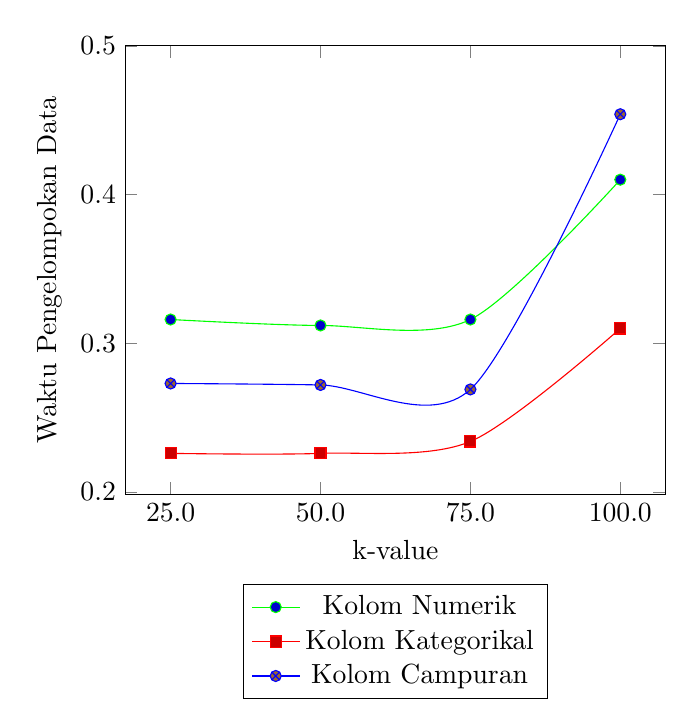
\begin{tikzpicture}[scale=\scl]
		\begin{axis}[\ymin,\ymax,xlabel=k-value, ylabel=Waktu Pengelompokan Data, xticklabel style={/pgf/number format/.cd, fixed,fixed zerofill, precision=1},ymax=0.50,xtick={25,50,75,100},legend style={at={(0.5,-0.2)},anchor=north}]
		\addlegendentry{Kolom Numerik}
		\addlegendentry{Kolom Kategorikal}
		\addlegendentry{Kolom Campuran}
		\addplot+[smooth][color=green] coordinates {(25,0.316) (50,0.312) (75,0.316) (100,0.41) };
		\addplot+[smooth][color=red] coordinates {(25,0.226) (50,0.226) (75,0.234) (100,0.31) };
		\addplot+[smooth][color=blue
		] coordinates {(25,0.273) (50,0.272) (75,0.269) (100,0.454) };
		\leg
		\end{axis}
		\end{tikzpicture}
		\captionsetup{justification=centering}
		\caption[Hasil 1]{Perubahan Waktu\\Pengelompokan Data}
		\label{fig:pengujian_column_1}
	\end{figure}
\end{minipage}
\begin{minipage}[c]{0.51\linewidth}
	\begin{figure}[H]
		\centering
		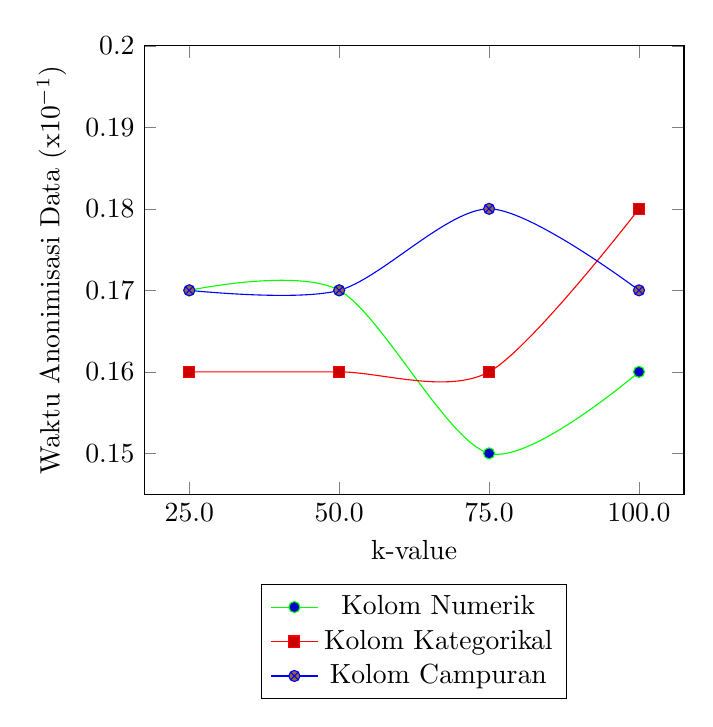
\begin{tikzpicture}[scale=\scl]
		\begin{axis}[\ymin,\ymax,xlabel=k-value,ylabel=Waktu Anonimisasi Data (x$10^{-1}$), xticklabel style={/pgf/number format/.cd, fixed,fixed zerofill, precision=1},ymax=0.20,xtick={25,50,75,100},legend style={at={(0.5,-0.2)},anchor=north}]
		\addlegendentry{Kolom Numerik}
		\addlegendentry{Kolom Kategorikal}
		\addlegendentry{Kolom Campuran}
		\addplot+[smooth][color=green] coordinates {(25,0.17) (50,0.17) (75,0.15) (100,0.16) };
		\addplot+[smooth][color=red] coordinates {(25,0.16) (50,0.16) (75,0.16) (100,0.18) };
		\addplot+[smooth][color=blue] coordinates {(25,0.17) (50,0.17) (75,0.18) (100,0.17) };
		\leg
		\end{axis}
		\end{tikzpicture}
		\captionsetup{justification=centering}
		\caption[Hasil 2]{Perubahan Waktu\\Anonimisasi Data}
		\label{fig:pengujian_column_2}
	\end{figure}
\end{minipage}\\

\begin{minipage}[c]{1\textwidth}
	\begin{figure}[H]
		\centering
		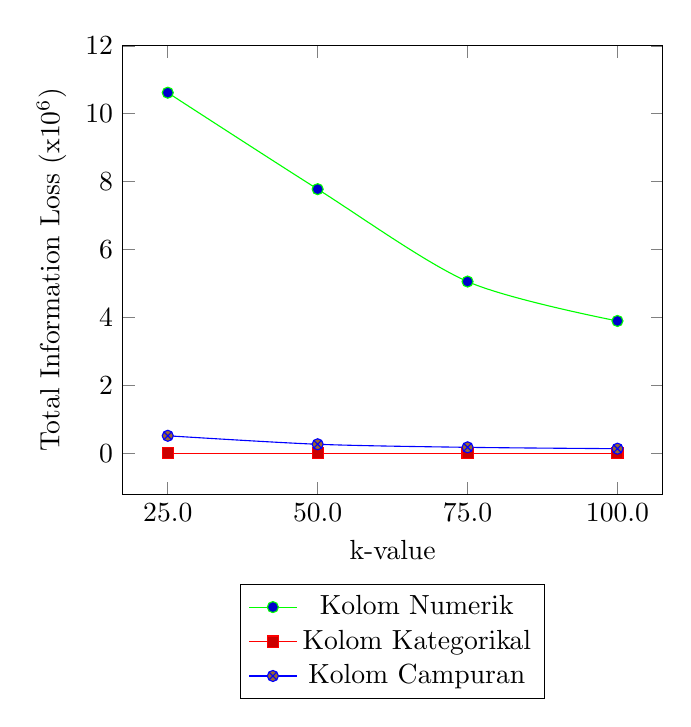
\begin{tikzpicture}[scale=\scl]
		\begin{axis}[\ymin,\ymax,xlabel= k-value,ylabel=Total Information Loss (x$10^{6}$), xticklabel style={/pgf/number format/.cd, fixed,fixed zerofill, precision=1},ymax=12,xtick={25,50,75,100},legend style={at={(0.5,-0.2)},anchor=north}]
		\addlegendentry{Kolom Numerik}
		\addlegendentry{Kolom Kategorikal}
		\addlegendentry{Kolom Campuran}
		\addplot+[smooth][color=green] coordinates {(25,10.62) (50,7.78) (75,5.06) (100,3.90) };
		\addplot+[smooth][color=red] coordinates {(25,0.002) (50,0.002) (75,0.002) (100,0.002) };
		\addplot+[smooth][color=blue] coordinates {(25,0.52) (50,0.27) (75,0.18) (100,0.14) };
		\leg
		\end{axis}
		\end{tikzpicture}
		\caption[Hasil 1]{Perubahan Total Information Loss}
		\label{fig:pengujian_column_3}
	\end{figure}
\end{minipage}

\begin{minipage}[t]{15.8cm}
\noindent \textbf{Kesimpulan:}\\
Berdasarkan pengujian jumlah kolom bervariasi diatas, diketahui bahwa hasil pengelompokan dengan algoritma greedy k-member clustering cukup baik jika menggunakan kolom campuran dengan pembobotan k-value = 100, karena memiliki total information paling kecil dari pengujian lainnya. Dari segi kecepatan komputasi, waktu pengelompokan data jauh lebih lama dibandingkan waktu anonimisasi karena beberapa pekerjaan pengelompokan data pada algoritma greedy k-member clustering tidak dapat dipecah secara paralel.
\end{minipage}

\vspace{0.5cm}
\textbf{Jumlah QID bervariasi}\\

\begin{minipage}[t]{15.8cm}
Tabel \ref{table:qid2}, \ref{table:qid3}, \ref{table:qid4} adalah contoh sampel pengujian berdasarkan pemilihan kolom numerik, kategorikal, kategorikal \& numerik dari dataset Credit score.
\end{minipage}

\begin{table}[h]
\centering
\caption{Sampel Data Credit score (|QID|=2)}
\vspace{0.1cm}
\begin{tabular}{|c|c|}
\hline 
DAYS\_BIRTH & OCCUPATION \\ 
\hline 
-12005 & Security staff \\ 
\hline 
-22464 & Sales staff \\ 
\hline 
-19110 & Sales staff \\ 
\hline 
\end{tabular} 
\label{table:qid2}
\end{table}  

\begin{table}[h]
\centering
\caption{Sampel Data Credit score (|QID|=3)}
\vspace{0.1cm}
\begin{tabular}{|c|c|c|}
\hline 
DAYS\_BIRTH & OCCUPATION & GENDER \\ 
\hline 
-12005 & Security staff & M \\ 
\hline 
-22464 & Sales staff & F \\ 
\hline 
-19110 & Sales staff & F \\ 
\hline 
\end{tabular} 
\label{table:qid3}
\end{table} 

\begin{table}[h]
\centering
\caption{Sampel Data Credit score (|QID|=4)}
\vspace{0.1cm}
\begin{tabular}{|c|c|c|c|}
\hline 
DAYS\_BIRTH & DAYS\_EMPLOYED & OCCUPATION & GENDER \\ 
\hline 
-12005 & -4542 & Security staff & M \\ 
\hline 
-22464 & -4542 & Sales staff & F \\ 
\hline 
-19110 & -769 & Sales staff & F \\ 
\hline 
\end{tabular} 
\label{table:qid4}
\end{table} 

\begin{minipage}[t]{15.8cm}
Pada pengujian ini, ingin dibuktikan apakah kualitas pengelompokan dan anonimisasi data dari algoritma greedy k-member clustering dan k-anonymity dapat diterima jika jumlah quasi-identifier bervariasi . Pengujian ini menggunakan |QIDs| $\in$ [2..4] dengan pengambilan 2 atribut numerik dan 2 atribut kategorikal, k $\in$ [25,50,75,100] terhadap n = 100. Berikut penjelasan jenis kajian yang diuji:
\end{minipage}\\

\begin{itemize}

\item \textbf{Clusterization Time}. Pengamatan ini dilakukan pada algoritma greedy k-member clustering. Gambar \ref{fig:pengujian_qid_2} menunjukkan waktu pengelompokan data mengalami peningkatan signifikan pada 3-QID dengan bobot k-value = 50. Selain itu, kolom 2-QID menempati waktu pengelompokan data tercepat dibandingkan 3-QID dan 4-QID. Melalui hasil pengujian ini, dapat ditarik kesimpulan bahwa pengelompokan data dapat dilakukan lebih cepat jika menggunakan sampel data dengan 2 quasi-identifier (2-QID) untuk setiap pembobotan k-value.

\item \textbf{Anonymization Time}. Pengamatan ini dilakukan pada algoritma k-anonymity. Gambar \ref{fig:pengujian_qid_2} menunjukkan waktu anonimisasi lebih lama pada penggunaan 4-QID. Hal ini dapat dilihat dari rentang waktu anonimisasi yang cukup besar antara 4-QID dengan 2-QID, 3-QID. Melalui hasil pengujian ini, dapat ditarik kesimpulan bahwa dengan bertambahnya kolom numerik pada sampel data dengan 4 quasi-idntifier (4-QID) memberikan pengaruh signifikan terhadap penambahan waktu anonimisasi. Proses anonimisasi juga memiliki waktu komputasi yang jauh lebih singkat dibandingkan pengelompokan data.


\item \textbf{Total Information Loss}. Pengamatan ini dilakukan pada algoritma greedy k-member clustering. Gambar \ref{fig:pengujian_qid_3} menunjukkan total information loss yang dihasilkan oleh 4-QID jauh lebih besar dibandingkan 2-QID dan 3-QID. Selain itu, total information loss mengalami penurunan seiring bertambahnya bobot k-value. Melalui hasil pengujian ini, dapat ditarik kesimpulan bahwa pengelompokan data dapat menghasilkan kualitas pengelompokan yang lebih baik jika total information loss yang dihasilkan kecil dengan menggunakan 2-QID, 3-OID dengan jumlah kolom numerik = 1 dan pembobotan k-value = 100.

\end{itemize}

\noindent
\begin{minipage}[c]{0.51\textwidth}
	\centering
	\begin{figure}[H]
		\centering
		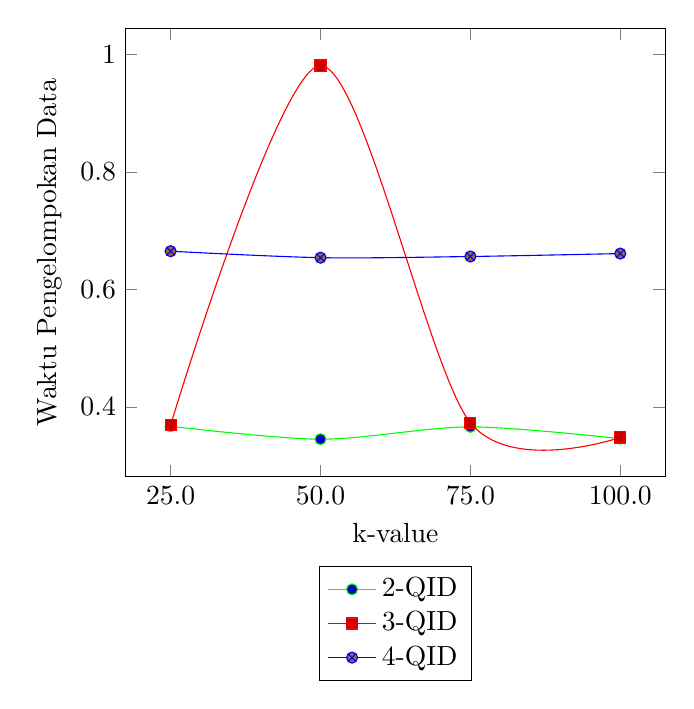
\begin{tikzpicture}[scale=\scl]
		\begin{axis}[\ymin,\ymax,xlabel= k-value,ylabel=Waktu Pengelompokan Data, xticklabel style={/pgf/number format/.cd, fixed,fixed zerofill, precision=1},xtick={25,50,75,100},legend style={at={(0.5,-0.2)},anchor=north}]
		\addlegendentry{2-QID}
		\addlegendentry{3-QID}
		\addlegendentry{4-QID}
		\addplot+[smooth][color=green] coordinates {(25,0.367) (50,0.345) (75,0.366) (100,0.346) };
		\addplot+[smooth][color=red] coordinates {(25,0.369) (50,0.981) (75,0.373) (100,0.348) };
		\addplot+[smooth][color=blue] coordinates {(25,0.665) (50,0.654) (75,0.656) (100,0.661) };
		\leg
		\end{axis}
		\end{tikzpicture}
		\captionsetup{justification=centering}
		\caption[Hasil 1]{Perubahan Waktu\\Pengelompokan Data}
		\label{fig:pengujian_qid_1}
	\end{figure}
\end{minipage}
\begin{minipage}[c]{0.51\linewidth}
	\begin{figure}[H]
		\centering
		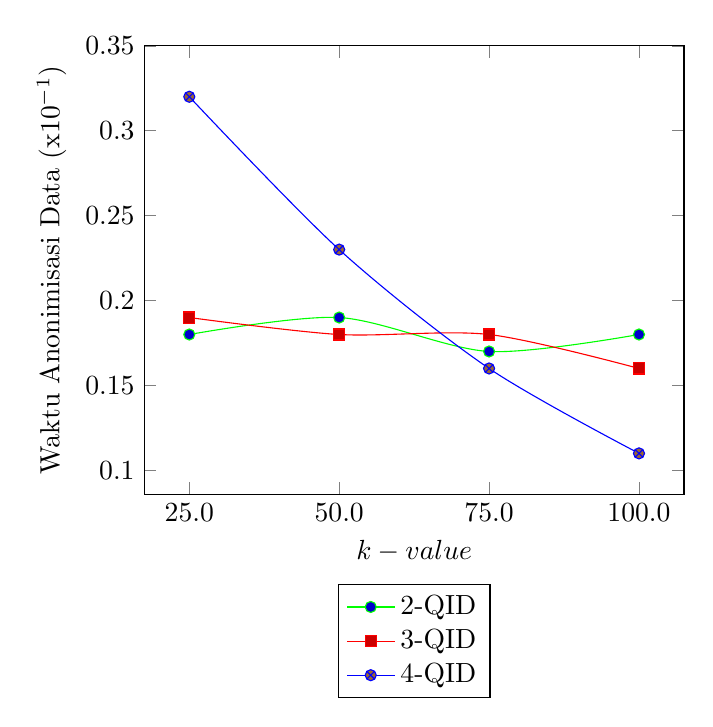
\begin{tikzpicture}[scale=\scl]
		\begin{axis}[\ymin,\ymax,xlabel=$k-value$,ylabel=Waktu Anonimisasi Data (x$10^{-1}$), xticklabel style={/pgf/number format/.cd, fixed,fixed zerofill, precision=1},ymax=0.35,xtick={25,50,75,100},legend style={at={(0.5,-0.2)},anchor=north}]
		\addlegendentry{2-QID}
		\addlegendentry{3-QID}
		\addlegendentry{4-QID}
		\addplot+[smooth][color=green] coordinates {(25,0.18) (50,0.19) (75,0.17) (100,0.18) };
		\addplot+[smooth][color=red] coordinates {(25,0.19) (50,0.18) (75,0.18) (100,0.16) };
		\addplot+[smooth][color=blue] coordinates {(25,0.32) (50,0.23) (75,0.16) (100,0.11) };
		\leg
		\end{axis}
		\end{tikzpicture}
		\captionsetup{justification=centering}
		\caption[Hasil 2]{Perubahan Waktu\\Anonimisasi Data}
		\label{fig:pengujian_qid_2}
	\end{figure}
\end{minipage}\\

\begin{minipage}[c]{1\textwidth}
	\begin{figure}[H]
		\centering
		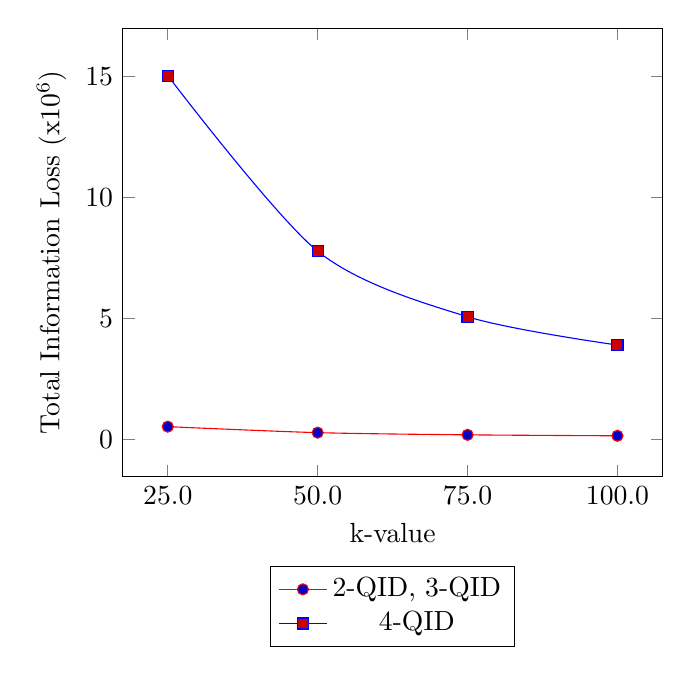
\begin{tikzpicture}[scale=\scl]
		\begin{axis}[\ymin,\ymax,xlabel= k-value,ylabel=Total Information Loss (x$10^{6}$), xticklabel style={/pgf/number format/.cd, fixed,fixed zerofill, precision=1},ymax=17,xtick={25,50,75,100},legend style={at={(0.5,-0.2)},anchor=north}]
		\addlegendentry{2-QID, 3-QID}
		\addlegendentry{4-QID}
		\addplot+[smooth][color=red] coordinates {(25,0.526) (50,0.278) (75,0.187) (100,0.148) };
		\addplot+[smooth][color=blue] coordinates {(25,15.04) (50,7.78) (75,5.07) (100,3.90) };
		\leg
		\end{axis}
		\end{tikzpicture}
		\caption[Hasil 1]{Perubahan Total Information Loss}
		\label{fig:pengujian_qid_3}
	\end{figure}
\end{minipage}

\begin{minipage}[t]{15.8cm}
\noindent \textbf{Kesimpulan:}\\
Berdasarkan pengujian jumlah QID bervariasi diatas, diketahui bahwa hasil pengelompokan dengan algoritma greedy k-member clustering cukup baik jika menggunakan 2-QID/3-QID dengan pembobotan k-value = 100, karena memiliki total information loss paling kecil dari pengujian lainnya. Dari segi kecepatan komputasi, waktu pengelompokan data jauh lebih lama dibandingkan waktu anonimisasi karena beberapa pekerjaan pengelompokan data pada algoritma greedy k-member clustering tidak dapat dikerjakan secara paralel.

\end{minipage}

\vspace{0.5cm}
\textbf{Ukuran data bervariasi}\\

\begin{minipage}[t]{15.8cm}
Tabel \ref{table:ukuran1} adalah sampel pengujian berdasarkan pemilihan kolom numerik, kategorikal, campuran dari dataset Credit score, dimana QID adalah quasi-identifier dan SA adalah sensitive attribute.
\end{minipage}

\begin{table}[h]
\centering
\caption{Sampel Data Credit score (10k dan 30k)}
\vspace{0.2cm}
\begin{tabular}{|c|c|c|}
\hline 
Nama Atribut & Tipe Data & Keterangan\\ 
\hline 
DAYS\_BIRTH & numerik & QID \\ 
\hline 
DAYS\_EMPLOYED & numerik & QID\\ 
\hline 
OCCUPATION\_TYPE & kategorikal & QID\\ 
\hline 
CODE\_GENDER & kategorikal & QID\\ 
\hline 
NAME\_INCOME\_TYPE & kategorikal & SA \\ 
\hline 
NAME\_EDUCATION\_TYPE & kategorikal & QID\\ 
\hline 
NAME\_FAMILY\_STATUS & kategorikal & QID\\ 
\hline 
NAME\_HOUSING\_TYPE & kategorikal & QID\\ 
\hline 
\end{tabular} 
\label{table:ukuran1}
\end{table} 

\vspace{0.5cm}
\begin{minipage}[t]{15.8cm}
Pada pengujian ini, ingin dibuktikan apakah kualitas pengelompokan dan anonimisasi data dari algoritma greedy k-member clustering dan k-anonymity dapat diterima jika ukuran data bervariasi . Pengujian ini menggunakan k $\in$ [25,50,75,100] dengan pengambilan atribut secara acak terhadap n = 10k dan n = 30k. Berikut penjelasan jenis kajian yang diuji:
\end{minipage}

\begin{itemize}

\item \textbf{Clusterization Time}. Pengamatan ini dilakukan pada algoritma greedy k-member clustering. Gambar \ref{fig:pengujian_uk_1} menunjukkan waktu pengelompokan data dengan n = 30k membutuhkan waktu dua kali lebih lama dibandingkan pengelompokan data dengan n = 10k, dengan total waktu pengelompokan data sekitar 10 jam. Selain itu, waktu pengelompokan data juga cenderung stabil seiring bertambahnya nilai k-value. Melalui hasil pengujian ini, dapat ditarik kesimpulan bahwa pengelompokan data dapat dilakukan lebih cepat jika menggunakan ukuran data yang relatif lebih kecil, yaitu n = 10k untuk setiap pembobotan k-value.

\item \textbf{Anonymization Time}. Pengamatan ini dilakukan pada algoritma k-anonymity. Gambar \ref{fig:pengujian_uk_2} menunjukkan proses anonimisasi dilakukan lebih lama pada sampel data n = 10k, dengan total waktu pengelompokan data sekitar 1.5 jam. Selain itu, k-value = 25 menempati posisi waktu anonimisasi data lebih tinggi dibandingkan dengan nilai k-value lainnya. Melalui hasil pengujian ini, dapat ditarik kesimpulan bahwa proses anonimisasi data dapat dilakukan lebih cepat jika menggunakan sampel ukuran data yang relatif kecil, yaitu n = 10k.

\item \textbf{Total Information Loss}. Pengamatan ini dilakukan pada algoritma greedy k-member clustering. Gambar \ref{fig:pengujian_uk_3} menunjukkan total information loss yang dihasilkan oleh n = 10k dan n = 30k hampir sama. Perbedaan signifikan total information loss hanya ditunjukan pada k-value = 25, dimana n = 10k menempati total information loss terkecil. Melalui hasil pengujian ini, dapat ditarik kesimpulan bahwa pengelompokan data dapat menghasilkan kualitas pengelompokan yang lebih baik jika total information loss yang dihasilkan kecil dengan menggunakan n = 10k maupun n = 30k untuk setiap pemilihan nilai k-value.
\end{itemize}

\noindent
\begin{minipage}[c]{0.51\textwidth}
	\centering
	\begin{figure}[H]
		\centering
		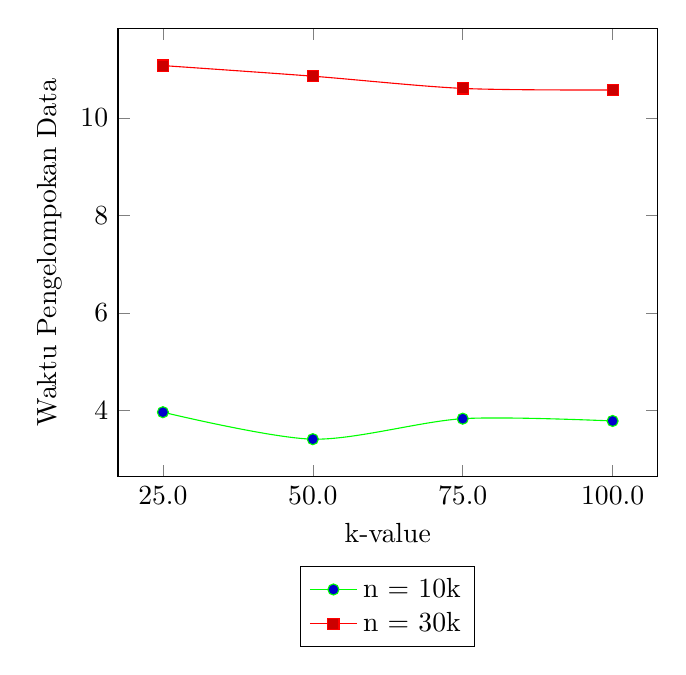
\begin{tikzpicture}[scale=\scl]
		\begin{axis}[\ymin,\ymax,xlabel= k-value,ylabel=Waktu Pengelompokan Data, xticklabel style={/pgf/number format/.cd, fixed,fixed zerofill, precision=1},xtick={25,50,75,100},legend style={at={(0.5,-0.2)},anchor=north}]
		\addlegendentry{n = 10k}
		\addlegendentry{n = 30k}
		\addplot+[smooth][color=green] coordinates {(25,3.9611) (50,3.4075) (75,3.828) (100,3.781) };
		\addplot+[smooth][color=red] coordinates {(25,11.0758) (50,10.858) (75,10.607) (100,10.575) };
		\leg
		\end{axis}
		\end{tikzpicture}
		\captionsetup{justification=centering}
		\caption[Hasil 1]{Perubahan Waktu\\Pengelompokan Data}
		\label{fig:pengujian_uk_1}
	\end{figure}
\end{minipage}
\begin{minipage}[c]{0.51\linewidth}
	\begin{figure}[H]
		\centering
		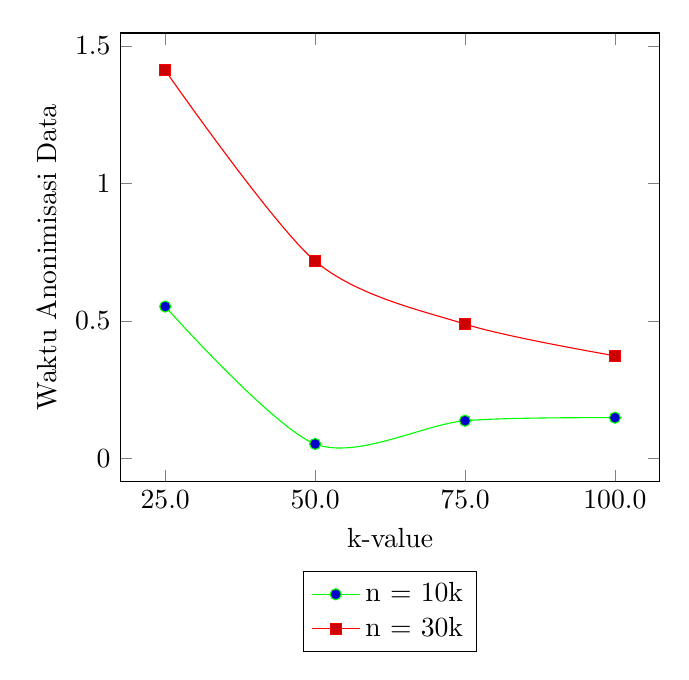
\begin{tikzpicture}[scale=\scl]
		\begin{axis}[\ymin,\ymax,xlabel=k-value,ylabel=Waktu Anonimisasi Data, xticklabel style={/pgf/number format/.cd, fixed,fixed zerofill, precision=1},xtick={25,50,75,100},legend style={at={(0.5,-0.2)},anchor=north}]
		\addlegendentry{n = 10k}
		\addlegendentry{n = 30k}
		\addplot+[smooth][color=green] coordinates {(25,0.5528) (50,0.0536) (75,0.138) (100,0.149) };
		\addplot+[smooth][color=red] coordinates {(25,1.4108) (50,0.7181) (75,0.489) (100,0.374) };
		\leg
		\end{axis}
		\end{tikzpicture}
		\captionsetup{justification=centering}
		\caption[Hasil 2]{Perubahan Waktu\\Anonimisasi Data}
		\label{fig:pengujian_uk_2}
	\end{figure}
\end{minipage}\\

\begin{minipage}[c]{1\textwidth}
	\begin{figure}[H]
		\centering
		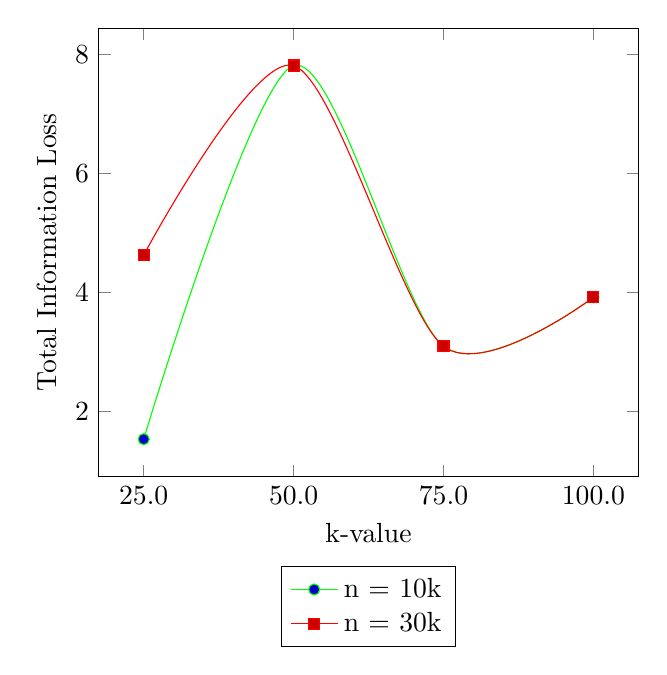
\begin{tikzpicture}[scale=\scl]
		\begin{axis}[\ymin,\ymax,xlabel= k-value,ylabel=Total Information Loss, xticklabel style={/pgf/number format/.cd, fixed,fixed zerofill, precision=1},xtick={25,50,75,100},legend style={at={(0.5,-0.2)},anchor=north}]
		\addlegendentry{n = 10k}
		\addlegendentry{n = 30k}
		\addplot+[smooth][color=green] coordinates {(25,1.54) (50,7.81) (75,3.10) (100,3.92) };
		\addplot+[smooth][color=red] coordinates {(25,4.63) (50,7.81) (75,3.10) (100,3.92) };
		\leg
		\end{axis}
		\end{tikzpicture}
		\caption[Hasil 1]{Perubahan Total Information Loss}
		\label{fig:pengujian_uk_3}
	\end{figure}
\end{minipage}
\vspace{0.5cm}

\begin{minipage}[t]{15.8cm}
\noindent \textbf{Kesimpulan:}\\
Berdasarkan pengujian jumlah QID bervariasi diatas, diketahui bahwa hasil pengelompokan dengan algoritma greedy k-member clustering cukup baik jika menggunakan ukuran data apapun dengan nilai k-value = 25, karena memiliki total information loss paling kecil dari pengujian lainnya. Dari segi kecepatan komputasi, waktu pengelompokan data jauh lebih lama dibandingkan waktu anonimisasi karena beberapa pekerjaan pengelompokan data pada algoritma greedy k-member clustering tidak dapat dikerjakan secara paralel. Hal penting yang perlu diketahui adalah komputasi pengelompokan data dengan n > 10k membutuhkan waktu lebih dari 3 jam sehingga diperlukan pertimbangan untuk menerapkan algortima greedy k-member clustering untuk lingkungan big data.
\end{minipage}

\newpage
\subsubsection{Pengujian Eksperimental Hasil Data Mining} 

Berikut adalah hasil setiap jenis pengujian eksperimental terhadap total informasi yang hilang:\\

\textbf{K-means}\\

\begin{minipage}[t]{15.8cm}
Pada pengujian ini, ingin dibuktikan apakah algoritma greedy k-member clustering dan k-anonymity dapat diterima jika hasil anonimisasinya digunakan untuk clustering/pengelompokan data. Pengujian ini menggunakan |QIDs| $\in$ [1..5] dengan pengambilan atribut secara acak terhadap n = 1000 dan k-value = 100, karena pada pengujian sebelumnya, kondisi ini memiliki information loss paling kecil. Berikut penjelasan jenis kajian yang diuji:
\end{minipage}

\begin{itemize}

\item \textbf{Silhouette score}. Pengamatan ini dilakukan dengan pemodelan k-means pada library Spark MLlib. Gambar \ref{fig:pengujian_km_1} menunjukkan silhouette score setelah anonimisasi stabil pada nilai 1. Perilaku ini disebabkan karena hasil anonimisasi yang pada cluster yang sejenis bernilai sama dan tidak dapat dibedakan satu sama lain. Hasil pengujian ini memberikan kesimpulan bahwa hasil pengelompokan setelah dilakukan anonimisasi lebih baik dibandingkan sebelum dilakukan anonimisasi, karena memiliki silhouette score yang lebih tinggi.

\item \textbf{Waktu komputasi}. Pengamatan ini dilakukan dengan komputer lokal (standalone). Gambar \ref{fig:pengujian_km_2} menunjukkan waktu komputasi tercepat untuk pembuatan model k-means didapat oleh data yang telah dianonimisasi. Perilaku ini disebabkan karena data yang telah dianonimisasi umumnya memiliki lebih sedikit jumlah variasi nilai, sehingga dapat mempercepat klasifikasi data. Hasil pengujian ini memberikan kesimpulan bahwa jumlah variasi nilai dapat memberi pengaruh terhadap waktu komputasi.

\item \textbf{Perbedaan hasil clustering ($\%$)}.  Pengamatan ini menghitung persentase perbedaan hasil clustering saat sebelum dan setelah data dianonimisasi pada kondisi jumlah data dan k yang beragam. Gambar \ref{fig:pengujian_km_3} menunjukkan persentase perbedaan hasil klasifikasi tertinggi berdasarkan nilai k diraih oleh $k=25,n=1000$. Gambar \ref{fig:pengujian_km_4} menunjukkan persentase perbedaan hasil klasifikasi tertinggi berdasarkan nilai k diraih oleh $k=10,n=1000$. Hasil dari pengujian ini memberikan kesimpulan bahwa nilai k yang semakin kecil dan ukuran data semakin besar dapat menyebabkan tingginya perbedaan hasil clustering.

\end{itemize}

\noindent
\begin{minipage}[c]{0.51\textwidth}
	\centering
	\begin{figure}[H]
		\centering
		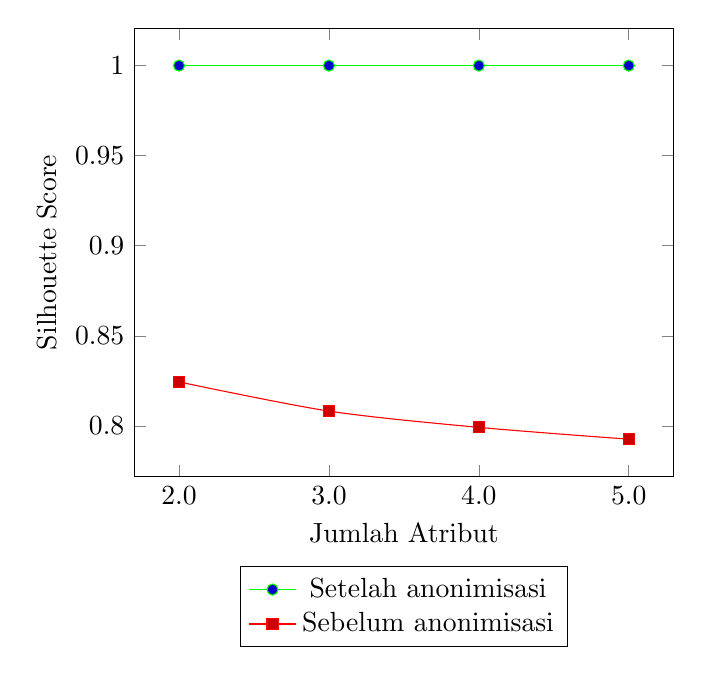
\begin{tikzpicture}[scale=\scl]
		\begin{axis}[\ymin,\ymax,xlabel= Jumlah Atribut,ylabel=Silhouette Score, xticklabel style={/pgf/number format/.cd, fixed,fixed zerofill, precision=1},xtick={2,3,4,5},legend style={at={(0.5,-0.2)},anchor=north}]
		\addlegendentry{Setelah anonimisasi}
		\addlegendentry{Sebelum anonimisasi}
		\addplot+[smooth][color=green] coordinates {(2,1.0) (3,1.0) (4,1.0) (5,1.0) };
		\addplot+[smooth][color=red] coordinates {(2,0.8244382495104136) (3,0.808251499166606) (4,0.7992133596986062) (5,0.7926606742596387) };
		\leg
		\end{axis}
		\end{tikzpicture}
		\captionsetup{justification=centering}
		\caption[Hasil 1]{Perbandingan Silhouette\\Score Model K-Means}
		\label{fig:pengujian_km_1}
	\end{figure}
\end{minipage}
\begin{minipage}[c]{0.51\linewidth}
	\begin{figure}[H]
		\centering
		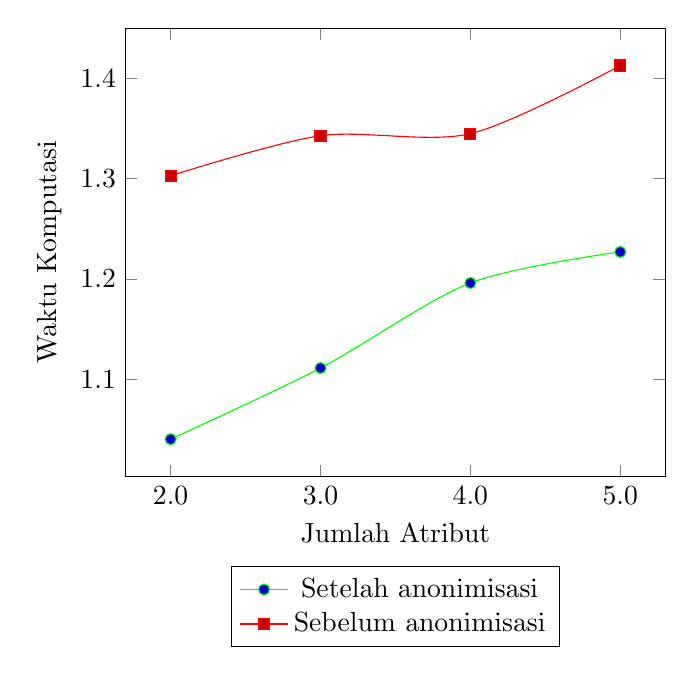
\begin{tikzpicture}[scale=\scl]
		\begin{axis}[\ymin,\ymax,xlabel=Jumlah Atribut,ylabel=Waktu Komputasi, xticklabel style={/pgf/number format/.cd, fixed,fixed zerofill, precision=1},xtick={2,3,4,5},legend style={at={(0.5,-0.2)},anchor=north}]
		\addlegendentry{Setelah anonimisasi}
		\addlegendentry{Sebelum anonimisasi}
		\addplot+[smooth][color=green] coordinates {(2,1.04) (3,1.111) (4,1.196) (5,1.227) };
		\addplot+[smooth][color=red] coordinates {(2,1.303) (3,1.343) (4,1.345) (5,1.413) };
		\leg
		\end{axis}
		\end{tikzpicture}
		\captionsetup{justification=centering}
		\caption[Hasil 2]{Perbandingan Waktu\\Komputasi Model K-Means}
		\label{fig:pengujian_km_2}
	\end{figure}
\end{minipage}\\

\noindent
\begin{minipage}[c]{0.51\textwidth}
	\centering
	\begin{figure}[H]
		\centering
		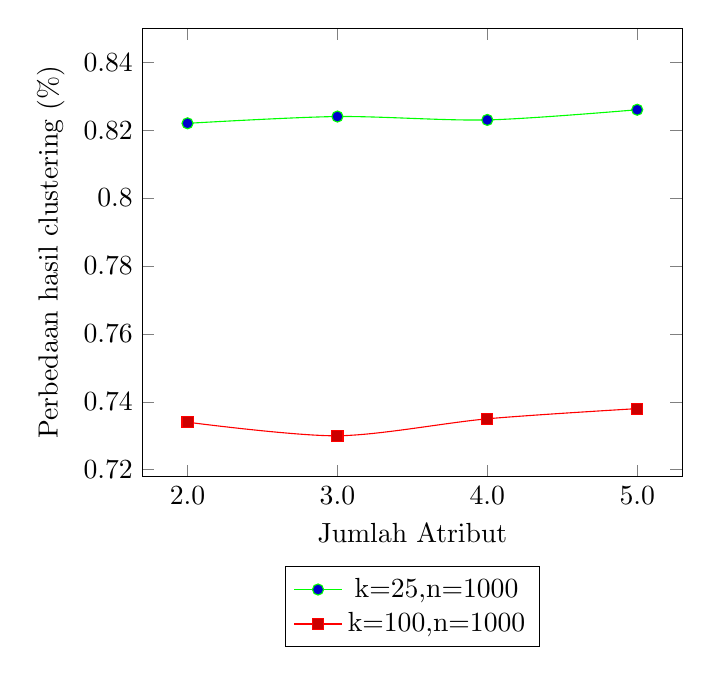
\begin{tikzpicture}[scale=\scl]
		\begin{axis}[\ymin,\ymax,xlabel= Jumlah Atribut,ylabel=Perbedaan hasil clustering ($\%$), xticklabel style={/pgf/number format/.cd, fixed,fixed zerofill, precision=1},ymax=0.85,xtick ={2,3,4,5},legend style={at={(0.5,-0.2)},anchor=north}]
		\addlegendentry{k=25,n=1000}
		\addlegendentry{k=100,n=1000}
		\addplot+[smooth][color=green] coordinates {(2,0.822) (3,0.824) (4,0.823) (5,0.826) };
		\addplot+[smooth][color=red] coordinates {(2,0.734) (3,0.73) (4,0.735) (5,0.738) };
		\leg
		\end{axis}
		\end{tikzpicture}
		\captionsetup{justification=centering}
		\caption[Hasil 1]{Perbandingan Hasil\\Clustering terhadap k}
		\label{fig:pengujian_km_3}
	\end{figure}
\end{minipage}
\begin{minipage}[c]{0.51\linewidth}
	\begin{figure}[H]
		\centering
		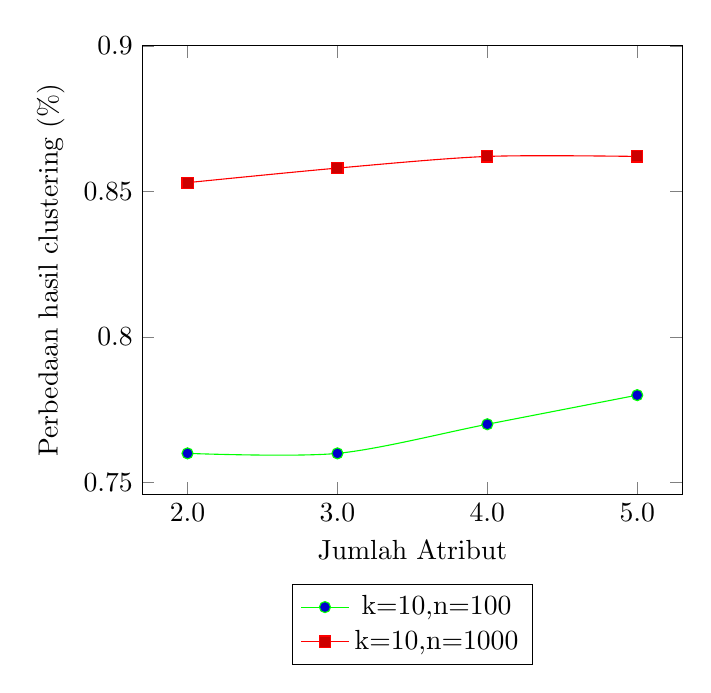
\begin{tikzpicture}[scale=\scl]
		\begin{axis}[\ymin,\ymax,xlabel=Jumlah Atribut,ylabel=Perbedaan hasil clustering ($\%$), xticklabel style={/pgf/number format/.cd, fixed,fixed zerofill, precision=1},ymax=0.90,xtick ={2,3,4,5},legend style={at={(0.5,-0.2)},anchor=north}]
		\addlegendentry{k=10,n=100}
		\addlegendentry{k=10,n=1000}
		\addplot+[smooth][color=green] coordinates {(2,0.76) (3,0.76) (4,0.77) (5,0.78) };
		\addplot+[smooth][color=red] coordinates {(2,0.853) (3,0.858) (4,0.862) (5,0.862) };
		\leg
		\end{axis}
		\end{tikzpicture}
		\captionsetup{justification=centering}
		\caption[Hasil 2]{Perbandingan Hasi\\Clustering terhadap n}
		\label{fig:pengujian_km_4}
	\end{figure}
\end{minipage}\\

\vspace{0.5cm}

\begin{minipage}[t]{15.8cm}
\noindent \textbf{Kesimpulan:}\\
Pada percobaan ini dapat disimpulkan 3 hal penting. Pertama, penggunaan algoritma greedy k-member clustering dan k-anonymity pada data credit score dapat diterima, karena hasil pengelompokannya sudah baik dibuktikan dengan hasil anonimisasi memiliki silhouette score bernilai 1. Kedua, penggunaan model k-means pada library Spark MLlib dapat melakukan komputasi dengan cepat untuk ukuran 1000 data. Ketiga, perbedaan hasil clustering paling minimal dapat dicapai dengan memperkecil ukuran data dan memperbesar nilai k

\end{minipage}

\vspace{0.5cm}
\textbf{Naive bayes}\\

\begin{minipage}[t]{15.8cm}
Pada pengujian ini, ingin dibuktikan apakah algoritma greedy k-member clustering dan k-anonymity dapat diterima jika hasil anonimisasinya digunakan untuk klasifikasi data. Pengujian ini menggunakan |QIDs| $\in$ [1..5] dengan pengambilan atribut secara acak terhadap n = 1000  dan k-value = 100, karena pada pengujian sebelumnya, kondisi ini memiliki information loss paling kecil. Berikut penjelasan jenis kajian yang diuji:
\end{minipage}

\begin{itemize}

\item \textbf{Tingkat akurasi}. Pengamatan ini dilakukan dengan pemodelan naive bayes pada library Spark MLlib. Gambar \ref{fig:pengujian_nb_1} menunjukkan perbedaan akurasi yang cukup tinggi (pada kondisi jumlah atribut berjumlah ganjil) dan perbedaan akurasi yang cukup dekat (pada kondisi jumlah atribut berjumlah genap). Perilaku ini disebabkan karena penyisipan jenis atribut bertipe numerik pada data dengan jumlah atribut genap. Hasil pengujian ini memberikan kesimpulan bahwa untuk mendapatkan tingkat akurasi yang baik, data yang digunakan perlu lebih banyak mengandung atribut numerik.

\item \textbf{Waktu komputasi}. Pengamatan ini dilakukan dengan komputer lokal (standalone). Gambar \ref{fig:pengujian_nb_2} menunjukkan waktu komputasi tercepat untuk pembuatan model naive bayes diraih oleh data yang telah dianonimisasi. Perilaku ini disebabkan karena data yang telah dianonimisasi umumnya memiliki lebih sedikit jumlah variasi nilai, sehingga dapat mempercepat klasifikasi data. Hasil pengujian ini memberikan kesimpulan bahwa jumlah variasi nilai dapat memberi pengaruh terhadap waktu komputasi.

\newpage
\item \textbf{Perbedaan hasil klasifikasi ($\%$)}. Pengamatan ini menghitung persentase perbedaan hasil klasifikasi saat sebelum dan setelah data dianonimisasi pada kondisi jumlah data yang beragam. Gambar \ref{fig:pengujian_nb_3} menunjukkan persentase perbedaan hasil klasifikasi tertinggi diraih oleh $n=1000$. Hasil dari pengujian ini memberikan kesimpulan bahwa jumlah data dapat mempengaruhi persentase perbedaan hasil klasifikasi, sehingga untuk mendapatkan perbedaan hasil klasifikasi yang minimal perlu mengurangi jumlah data yang diuji.

\end{itemize}

\noindent
\begin{minipage}[c]{0.51\textwidth}
	\centering
	\begin{figure}[H]
		\centering
		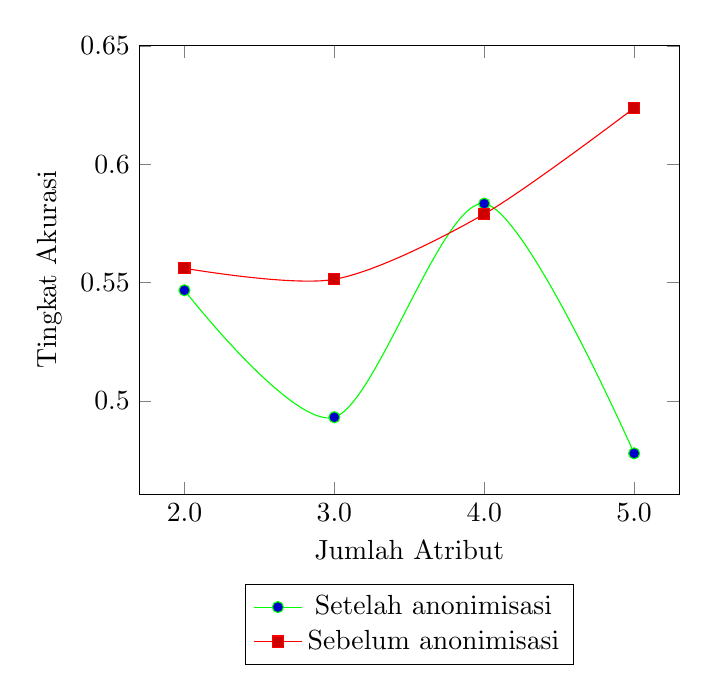
\begin{tikzpicture}[scale=\scl]
		\begin{axis}[\ymin,\ymax,xlabel= Jumlah Atribut,ylabel=Tingkat Akurasi, xticklabel style={/pgf/number format/.cd, fixed,fixed zerofill, precision=1},ymax=0.65,xtick ={2,3,4,5},legend style={at={(0.5,-0.2)},anchor=north}]
		\addlegendentry{Setelah anonimisasi}
		\addlegendentry{Sebelum anonimisasi}
		\addplot+[smooth][color=green] coordinates {(2,0.5467289719626168) (3,0.4930875576036866) (4,0.5833333333333334) (5,0.4778325123152709) };
		\addplot+[smooth][color=red] coordinates {(2,0.5560344827586207) (3,0.5513513513513514) (4,0.5789473684210527) (5,0.6237113402061856) };
		\leg
		\end{axis}
		\end{tikzpicture}
		\captionsetup{justification=centering}
		\caption[Hasil 1]{Perbandingan Tingkat\\Akurasi Model Naive Bayes}
		\label{fig:pengujian_nb_1}
	\end{figure}
\end{minipage}
\begin{minipage}[c]{0.51\textwidth}
	\begin{figure}[H]
		\centering
		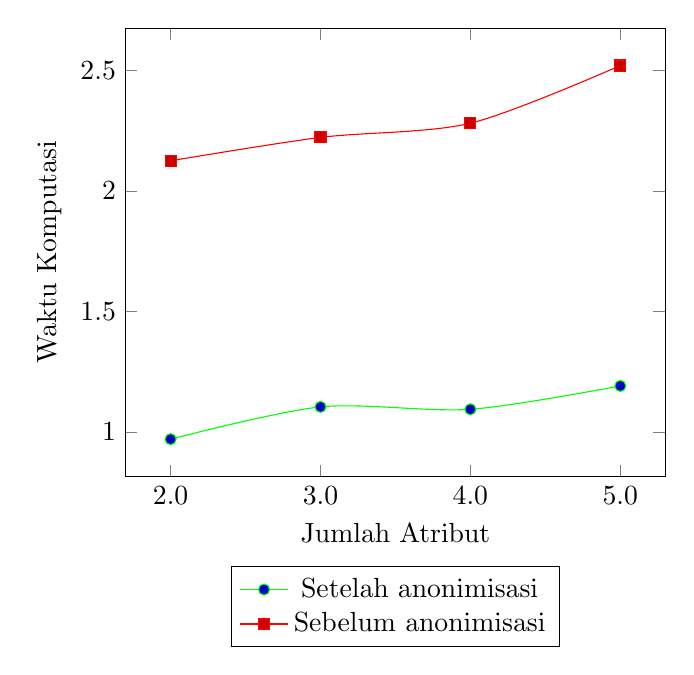
\begin{tikzpicture}[scale=\scl]
		\begin{axis}[\ymin,\ymax,xlabel=Jumlah Atribut,ylabel=Waktu Komputasi, xticklabel style={/pgf/number format/.cd, fixed,fixed zerofill, xtick ={2,3,4,5}, precision=1},legend style={at={(0.5,-0.2)},anchor=north}]
		\addlegendentry{Setelah anonimisasi}
		\addlegendentry{Sebelum anonimisasi}
		\addplot+[smooth][color=green] coordinates {(2,0.97) (3,1.104) (4,1.094) (5,1.191) };
		\addplot+[smooth][color=red] coordinates {(2,2.125) (3,2.222) (4,2.281) (5,2.52) };
		\leg
		\end{axis}
		\end{tikzpicture}
		\captionsetup{justification=centering}
		\caption[Hasil 2]{Perbandingan Waktu\\Komputasi Model Naive Bayes}
		\label{fig:pengujian_nb_2}
	\end{figure}
\end{minipage}\\

\begin{minipage}[c]{1\textwidth}
	\begin{figure}[H]
		\centering
		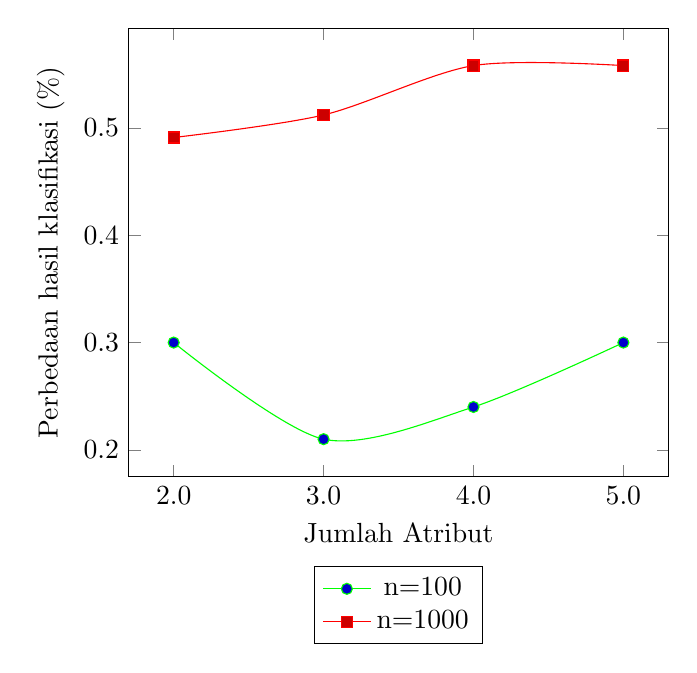
\begin{tikzpicture}[scale=\scl]
		\begin{axis}[\ymin,\ymax,xlabel=Jumlah Atribut,ylabel=Perbedaan hasil klasifikasi ($\%$), xticklabel style={/pgf/number format/.cd, fixed,fixed zerofill, xtick ={2,3,4,5}, precision=1},legend style={at={(0.5,-0.2)},anchor=north}]
		\addlegendentry{n=100}
		\addlegendentry{n=1000}
		\addplot+[smooth][color=green] coordinates {(2,0.3) (3,0.21) (4,0.24) (5,0.3) };
		\addplot+[smooth][color=red] coordinates {(2,0.491) (3,0.512) (4,0.558) (5,0.558) };
		\leg
		\end{axis}
		\end{tikzpicture}
		\captionsetup{justification=centering}
		\caption[Hasil 2]{Perbedaan Hasil Klasifikasi\\terhadap Jumlah Data}
		\label{fig:pengujian_nb_3}
	\end{figure}
\end{minipage}\\

\vspace{0.5cm}

\begin{minipage}[t]{15.8cm}
\noindent \textbf{Kesimpulan:}\\
Pada percobaan ini dapat disimpulkan 3 hal penting. Pertama, penggunaan algoritma greedy k-member clustering dan k-anonymity pada data credit score dapat diterima, karena pada kasus tertentu tingkat akurasi sebelum dan setelah anonimisasi memiliki perbedaan cukup dekat. Kedua, penggunaan model naive bayes pada library Spark MLlib dapat melakukan komputasi dengan cepat untuk ukuran 1000 data. Ketiga, perbedaan hasil klasifikasi paling minimal dapat dicapai dengan memperkecil ukuran data pengujian.
\end{minipage}

\subsubsection{Kesimpulan Pengujian Eksperimental} 

Beberapa hal penting yang perlu dipertimbangkan untuk penelitian selanjutnya. Pertama, pengelompokan data dengan greedy k-member clustering sangat lama sehingga dapat diganti ke library KMeans milik Spark MLlib. Kedua, total information loss dapat diminimalisir dengan penggunaan nilai k-value yang cukup besar dan jumlah quasi-identifier secukupnya. Ketiga, metode data mining terbaik untuk hasil anonimisasi adalah klasifikasi karena menghasilkan perbedaan prediksi paling sedikit. Hasil pengujian dapat dilihat pada Tabel \ref{table:kesimpulan_eksperimen}.

\noindent
\begin{table}[h]
\centering
\caption{Kesimpulan Pengujian Eksperimental}
\vspace{0.1cm}
\begin{tabular}{|p{3cm}|p{3cm}|p{3cm}|p{5.5cm}|}
    \hline
    \textbf{\newline Hasil\newline Pengujian} & \textbf{\newline Kajian} & 	  \textbf{\newline Parameter\newline Terbaik \newline} & \textbf{\newline Kesimpulan} \\
    \hline
    \multirow{3}{*}{\parbox{3cm}{Total \newline Information Loss}} & \parbox{3cm}{\vspace{0.5cm} column \newline} & kolom campuran,\newline k-value = 100 & Parameter ini dipilih karena memiliki total information loss paling kecil yaitu kurang dari $(2\times10^{6})$ untuk 1000 data.\\ \cline{2-4}
     & \parbox{3cm}{\vspace{0.5cm} |QIDs| \newline} & 2-QID/3-QID,\newline 1 kolom numerik, 2 kolom kategori,\newline k-value = 100  & Parameter ini dipilih karena memiliki total information loss paling kecil yaitu kurang dari $(1\times10^{6})$ untuk 1000 data.\\ \cline{2-4}
     & \parbox{3cm}{\vspace{0.5cm} size \newline} & 7-QID,\newline 2 kolom numerik, 5 kolom kategori,\newline k-value = 25 & Parameter ini dipilih karena memiliki total information loss paling kecil yaitu kurang dari $(4\times10^{7})$ untuk 10.000 data. \\ 
    \hline
    \multirow{2}{*}{\parbox{3cm}{\vspace{0.5cm} Hasil \newline Data Mining}} & \parbox{3cm}{\vspace{0.5cm} k-means \newline} & k = 100,\newline n = 100 & Parameter ini dipilih karena memiliki perbedaan hasil clustering terendah (0.74) terhadap data sebelum dan setelah anonimisasi.\newline \\ \cline{2-4}
     & \parbox{3cm}{\vspace{0.5cm} naive bayes \newline} & n = 100 & Parameter ini dipilih karena memiliki perbedaan hasil klasifikasi terendah (0.30) terhadap data sebelum dan setelah anonimisasi  \\
    \hline
    \end{tabular}
\label{table:kesimpulan_eksperimen}
\end{table}
